\part{Monitoring}
\label{partIII}

\chapter{\acrlong{S-MAB} Algorithms}
\glsresetall
\label{chapter:S-MAB}

The content of this chapter bases on the following publication: 
\begin{itemize}[noitemsep]
	\item \fullcite{DBLP:conf/kdd/FoucheKB19}
\end{itemize}
\textbf{Keywords:} Bandit Algorithms; Thompson Sampling; Adaptive Windowing%; Data Stream Monitoring; Predictive Maintenance

\section{Chapter Overview}

The \gls{MAB} is a fundamental model capturing the dilemma between exploration and exploitation in sequential decision-making. 
At every time step, the decision-maker selects a set of arms and observes a reward from each of the chosen arms. 
In this chapter, we present a variant of the problem, which we call the \gls{S-MAB}: the goal of the decision-maker is not only to maximise the cumulative rewards, i.e., choosing the arms with the highest expected reward, but also to decide how many arms to select so that, in expectation, the cost of selecting arms does not exceed the rewards. 
This problem is relevant to many real-world applications, e.g., online advertising, financial investments or data stream monitoring. In Section \ref{section:notationsbandits}, we introduced the required notation to describe and analyse our algorithms. This chapter makes the following contributions:  

\textbf{We address the \gls{S-MAB} problem, a novel generalisation of the \gls{MAB} problem.} The novelty is that the decision-maker not only decides which arms to play, but also how many, to maximise her cumulative reward under an efficiency constraint. 
To our knowledge, we are the first to consider this setting.   

\textbf{We first propose \gls{S-TS}, an algorithm to solve this problem in the static setting}, i.e., when the distribution of rewards does not change over time. 
We leverage existing bandit algorithms, e.g., \gls{TS}, and show that the regret of our method (i.e., the difference from the outcome of a perfect oracle) %EF: Note that here we do not only talk about expected rewards, regret in our case is also "pull regret" so "outcome" is more general.
only grows logarithmically with the number of time steps. 

\textbf{Then, we generalise our method for the non-static setting.} To do so, we combine our algorithm with \gls{ADWIN}, a state-of-the-art change detector, which is at the same time efficient and offers theoretical guarantees. 

\textbf{Finally, we validate our findings via experiments.} We illustrate the benefits of our contribution via a real-world use case on predictive maintenance. The comparison with existing approaches shows that our method achieves state-of-the-art results. 
-- We release our source code and data on GitHub\footnote{\url{https://github.com/edouardfouche/S-MAB}}, to ensure reproducibility.

\section{\acrlong{S-TS}}
\label{sec:STS}

Let us first assume a static environment. Our algorithm consists of: 
\begin{enumerate}[noitemsep]
	\item A \gls{MP-MAB} to identify the top-$\gls{L}_{\gls{t}}$ arms (\hyperlink{*1}{\textbf{*1}}). \label{component1}
	\item A so-called `scaling policy', to determine the value of $\gls{L}_{\gls{t}+1}$ based on $\gls{L}_{\gls{t}}$ and the observations at time $\gls{t}$ (\hyperlink{*2}{\textbf{*2}}). \label{component2}
\end{enumerate}

For (\ref{component1}), we use an existing algorithm, \gls{MP-TS}. It is a Bayesian-inspired bandit algorithm, which maintains a Beta posterior with parameters $\alpha_i, \beta_i$ over each arm $i$. In each round, \gls{MP-TS} samples an observation $\theta_i$ from each posterior and selects the top-$\gls{L}_{\gls{t}}$ arms according to these observations. Then, the parameters of this posterior are adjusted based on the reward vector $\gls{X(t)}$. 

%Our experiments (Section \ref{evaluation}) will show that MP-TS yields better results than MP-MAB based on UCB \cite{Chen2016}, KL-UCB \cite{garivier2018kl} and Exp3 \cite{auer1995gambling}. 

For (\ref{component2}), we propose to use a scaling policy, i.e., a strategy to control the number of plays, such that the empirical efficiency $\hat{\eta}_{\gls{t}}$ remains larger than $\gls{eta^*}$. Whenever $\hat{\eta}_{\gls{t}} \leq \gls{eta^*}$, we `scale down', i.e., we set $\gls{L}_{\gls{t}+1} = \gls{L}_{\gls{t}} - 1$. Otherwise, we `scale up'. 
When we are confident that adding one arm will lead to $\hat{\eta}_{\gls{t}} \leq \gls{eta^*}$, we stop scaling. 
To do so, we estimate $B_{\gls{t}}$, an upper confidence bound for $\hat{\eta}_{\gls{t}+1}$, assuming that $\gls{L}_{\gls{t}+1} = \gls{L}_{\gls{t}} + 1$. $\hat{B}_{\gls{t}}$ is our estimator for $B_{\gls{t}}$, based on the observations from the environment so far. The confidence is derived from the Kullback-Leibler divergence, as the so-called \gls{KL-UCB} index \cite{DBLP:journals/jmlr/GarivierC11,DBLP:conf/alt/Maillard17}. 
We name our policy  \gls{KL-S}:
\begin{align}
\label{scalingpolicy_analysis}
\gls{L}_{\gls{t}+1} = 
\begin{cases}
\gls{L}_{\gls{t}}-1 
&\quad\text{if } \hat{\eta}_{\gls{t}}  \leq  \gls{eta^*}  \\
\gls{L}_{\gls{t}}+1
&\quad\text{if } \hat{\eta}_{\gls{t}} >  \gls{eta^*} \text{ and } \hat{B}_{\gls{t}} >  \gls{eta^*}\\ 
\gls{L}_{\gls{t}}
&\quad\text{otherwise} \\ 
\end{cases}
\end{align}
where $1 \leq \gls{L}_{\gls{t}+1} \leq  \gls{K}$ and
\begin{align}
\hat{\eta}_{\gls{t}} = \frac{1}{\gls{L}_{\gls{t}}} \sum_{i}^{\gls{I(t)}} \hat{\mu}_i &&
\hat{B}_{\gls{t}} = \frac{\gls{L}_{\gls{t}}}{\gls{L}_{\gls{t}}+1} \hat{\eta}_{\gls{t}} + \frac{1}{\gls{L}_{\gls{t}}+1} b_{\widehat{\gls{L}_{\gls{t}}+1}}(\gls{t})
\end{align}
$\hat{B}_{\gls{t}}$ is the empirical estimator of 
\[
B_{\gls{t}} = \frac{1}{\gls{L}_{\gls{t}}+1} \sum_{i=1}^{\gls{L}_{\gls{t}}} \gls{mu_i}(\gls{t}) + \frac{1}{\gls{L}_{\gls{t}}+1} b_{\gls{L}_{\gls{t}}+1}(\gls{t}).
\] 
where $b_i(\gls{t})$ is the  \gls{KL-UCB} index of arm $i$ and $\widehat{\gls{L}_{\gls{t}}+1}$ is the arm of the ($\gls{L}_{\gls{t}}+1$)-th largest index. The  \gls{KL-UCB} index is as follows: 
\begin{equation}
\label{kl-index}
b_i(\gls{t}) = \max_q \{  \gls{N_i(t)} \cdot d_{\text{KL}}(\hat{\mu}_i(\gls{t}), q) \le \log(\gls{t}/ \gls{N_i(t)})\}
\end{equation}
where $d_{\text{KL}}$ is the Kullback-Leibler divergence. Intuitively, our policy maximises $\gls{L}_{\gls{t}}$ such that the empirical efficiency $\hat{\eta}_{\gls{t}}$ remains larger than $ \gls{eta^*}$ at any time $\gls{t}$. We stop scaling up whenever $\hat{B}_{\gls{t}}$, which is an upper confidence bound of $\hat{\eta}_{\gls{t}}$, is greater than $ \gls{eta^*}$.

In  \gls{S-TS}, the algorithms of (\ref{component1})  \gls{MP-TS} and (\ref{component2})  \gls{KL-S} are intertwined. 
See Algorithm \ref{S-TS}.   \gls{S-TS} successively calls the two procedures  \gls{MP-TS} and  \gls{KL-S}, 
while maintaining the statistics $\gls{N_i(t)}, \gls{S_i(t)}$ for each arm. 
We initialise the scaling policy with $\gls{L}_1 =  \gls{K}$ (Lines~\ref{alg1line1}-\ref{alg1line2}).
The rationale is that nothing is known about the reward distribution of the arms initially, so pulling a maximum number of arms is informative. Previous studies showed that optimistic initialisation improves the empirical performance of bandit algorithms \cite{DBLP:journals/corr/KuleshovP14, DBLP:books/lib/SuttonB98}. 

\textbf{Computational complexity of Algorithm \ref{S-TS}:}
At each round,  \gls{MP-TS} draws a sample from a Beta distribution (Line \ref{betadrawing}), and  \gls{KL-S} computes the  \gls{KL-UCB} index for each arm (Line \ref{klindex-computation}), which can be done efficiently via Newton's method. 
Given that these operations are done in constant time and that finding the top-$\gls{L}_{\gls{t}}$ elements among $ \gls{K}$ elements takes $O( \gls{K} \log  \gls{K})$ in the worst case ($\gls{L}_{\gls{t}} =  \gls{K}$), each round of the proposed algorithm takes $O( \gls{K} \log  \gls{K})$ time. Therefore, the total computational complexity of the algorithm is $O(\gls{T} \gls{K} \log(\gls{K}))$.
The space complexity of the algorithm is $O( \gls{K})$, as it only keeps four statistics ($\alpha_i$, $\beta_i$, $N_i$, $S_i$) per arm $i \in [ \gls{K}]$. 

\begin{algorithm}
	\footnotesize
	\caption{ \gls{S-TS}($[\gls{K}], \eta^*$)}\label{S-TS} 
	\begin{algorithmic}[1]
		\Require Set of arms
		$[\gls{K}] = \{1,2,\dots, \gls{K}\}$, target efficiency $ \gls{eta^*}$
		\State $\alpha_i(1) = 0$, $\beta_i(1) = 0$ \quad $\forall i \in [ \gls{K}]$ \label{alg1line1}
		\State $N_i(1) = 0$, $S_i(1) = 0$ \quad $\forall i \in [ \gls{K}]$  \label{alg1line2}
		\State $\gls{L}_1 \gets  \gls{K}$ 
		\For{$t = 1,2,\dots,\gls{T}$}
		\State $ \gls{I(t)},  \gls{X(t)} \gets $ \Call{ \gls{MP-TS}}{$\gls{L}_{\gls{t}}$} \Comment{Play $\gls{L}_{\gls{t}}$ arms (as in  \gls{MP-TS})}
		\For{$i \in  \gls{I(t)}$}
		\State $N_i(\gls{t}+1) =  \gls{N_i(t)} + 1$
		\State $S_i(\gls{t}+1) =  \gls{S_i(t)} +  \gls{X_i(t)}$
		\EndFor
		\State $\gls{L}_{\gls{t}+1} \gets$ \Call{ \gls{KL-S}}{$\gls{L}_{\gls{t}}$} \Comment{Scale $\gls{L}_{\gls{t}}$ for the next round}
		\EndFor
		\Statex~
		\Procedure{ \gls{MP-TS}}{$\gls{L}_{\gls{t}}$} \label{line_mpts}
		\For{$i = 1,\dots, \gls{K}$}  
		\State $\theta_i(\gls{t}) \sim \text{Beta}(\alpha_i(\gls{t})+1, \beta_i(\gls{t})+1)$ \label{betadrawing}
		\EndFor 
		\State Play arms $ \gls{I(t)} := \argmax_{K' \subset [ \gls{K}], |K'| = \gls{L}_{\gls{t}}} \sum_{i}^{K'}\theta_i(\gls{t})$ \label{sorting-theta}
		\State Observe reward vector $ \gls{X(t)}$
		\For{$i \in  \gls{I(t)}$} \Comment{Update parameters}
		\State $\alpha_i(\gls{t}+1) = \alpha_i(\gls{t}) +  \gls{X_i(t)}$ 
		\State $\beta_i(\gls{t}+1) = \beta_i(\gls{t}) + (1- \gls{X_i(t)})$ 
		\EndFor
		\State \textbf{return} $ \gls{I(t)},  \gls{X(t)}$
		\EndProcedure
		\Statex~
		\Procedure{ \gls{KL-S}}{$\gls{L}_{\gls{t}}$}
		\State $S_i = S_i(\gls{t}+1), N_i = N_i(\gls{t}+1) \quad \forall i \in [ \gls{K}]$
		\State $\hat{\mu}_i = S_i/N_i \quad \forall i \in [ \gls{K}]$ \Comment{$\hat{\mu}_i = 1$, if $N_i = 0$}
		\State $\hat{\eta}_{\gls{t}} = \sum_{i \in  \gls{I(t)}} \hat{\mu}_i$
		\If{$\hat{\eta}_{\gls{t}} \leq  \gls{eta^*}$} \textbf{return} $\max(\gls{L}_{\gls{t}} - 1, 1) $
		\Comment{Scale down}
		\Else{
			\State  $KL = \left \{	\max_q \{ N_i\cdot d_{\text{KL}}(\hat{\mu}_i, q) \le \log\frac{\gls{t}+1}{N_i}\}: \forall i \in [ \gls{K}] \right\}$ \label{klindex-computation}
			\State $b_{\widehat{\gls{L}_{\gls{t}} +1}} = (\gls{L}_{\gls{t}} + 1)$-th largest element from $KL$ \label{sorting-kl}
			\State $\hat{B}_{\gls{t}}$ = $\frac{\gls{L}_{\gls{t}}}{\gls{L}_{\gls{t}} + 1} \hat{\eta}_{\gls{t}} + \frac{1}{\gls{L}_{\gls{t}} + 1} b_{\widehat{\gls{L}_{\gls{t}} + 1}}(\gls{t})$
			\If{$\hat{B}_{\gls{t}} >  \gls{eta^*}$}  \textbf{return} $\min(\gls{L}_{\gls{t}} + 1,  \gls{K})$ \Comment{Scale up}
			\Else ~\textbf{return} $\gls{L}_{\gls{t}}$ \Comment{Do not scale}
			\EndIf
		}
		\EndIf
		\EndProcedure
	\end{algorithmic}
\end{algorithm}

\section{\acrlong{S-TS-ADWIN}}
\label{non-static-adaptation}

To handle the non-static setting (\hyperlink{*3}{\textbf{*3}}), we combine  \gls{S-TS} with \gls{ADWIN} \cite{DBLP:conf/sdm/BifetG07}. We call the resulting algorithm \gls{S-TS-ADWIN}.

\gls{ADWIN} (Algorithm \ref{ADWIN}) monitors the expected value from a single (virtually infinite) stream of values $\{x_1,x_2,\dots\}$, where $x_i \in [0,1]$. 
\gls{ADWIN} maintains a window $W$ of varying size $|W| = \gls{w}$ so that the nature of the stream is consistent. \gls{ADWIN} reduces the size of the window whenever two neighbouring subwindows have different mean, based on a statistical test with %a given
confidence $\delta$. %Let $t$ be the current time step. 
For every two subwindows of size $|W_1| + |W_2| = |W|$ with corresponding means $\hat{\mu}_{W_1},\hat{\mu}_{W_2}$, \gls{ADWIN} shrinks the windows to $W_2$ if 
\begin{equation}
 |\hat{\mu}_{W_1} - \hat{\mu}_{W_2}| \ge \epsiloncut^\delta \quad \mathrm{where} \quad \epsiloncut^\delta = \sqrt{\frac{1}{2 m} \log\left(\frac{4 |W|}{\delta}\right)}
\end{equation}
and $m = 1/((1/|W_1|)+(1/|W_2|))$. %EF: We don't need the detail on \delta' (simpler)
\cite{DBLP:conf/sdm/BifetG07} showed that \gls{ADWIN} efficiently adapts to both gradual and abrupt changes with theoretical guarantees %on the rates of false positives and false negatives 
(see Theorem 3.1 therein).

\begin{algorithm}
	\footnotesize
	\caption{\gls{ADWIN}($B$, $\delta$)}\label{ADWIN} 
	\begin{algorithmic}[1]
		\Require Stream of values $B = (x_{1}, x_{2}, \dots)$, confidence level $\delta$ 
		\State $W \leftarrow \{\}$
		\For{$t = 1,2,\dots$}
		\State $W \leftarrow W \cup \{x_{\gls{t}}\}$
		\State Drop elements from the tail of $W$ until $|\hat{\mu}_{W_1} - \hat{\mu}_{W_2}| < \epsiloncut^\delta$ holds for every split $W = W_1 \cup W_2$. 
		\EndFor
	\end{algorithmic}
\end{algorithm}

The idea behind \gls{S-TS-ADWIN}, showed in Algorithm \ref{S-TS-ADWIN}, is to create an \gls{ADWIN}  instance $A_i$ per arm $i$.
At each step $t$, $A_i$ obtains as input the reward from the corresponding arm $\gls{X_i(t)}$ if $i \in \gls{I(t)}$. 
Thus, each instance $A_i$ maintains a time window $W_i$ of variable size, which shrinks whenever \gls{ADWIN} detects a change in $\gls{mu_i}$.  

However, for any bandit algorithm with logarithmic regret, the number of plays of suboptimal arms grows with $\log(\gls{T})$. 
That is, after some time, the $A_j$ of any suboptimal arm $j$ does not obtain any input, and thus no change can be detected for arm $j$. 

Thus, we use $\gls{w}_{\gls{t}} = \min\{|W_i|: \forall i \in [\gls{K}]\}$, i.e., the smallest window from each $A_i$, to estimate the statistics of any arm~$i \in [\gls{K}]$ at each step $\gls{t}$. 
Here, we implicitly assume that the change points are `global', i.e., that they are shared across the $\gls{mu_i}, \forall i \in [\gls{K}]$. In principle, changes may also be `local', e.g., a single $\gls{mu_i}$ changes. But we will show that despite this assumption, it works well in practice. %EF: That is not completely exact. It works well in our synthetic examples because the arms changing are top-arms. This would be a different story if suddenly suboptimal arm would become optimal. 

\begin{algorithm} 
	\footnotesize
	\caption{\acrshort{S-TS-ADWIN}($[\gls{K}], \gls{eta^*}, \delta$)}\label{S-TS-ADWIN} 
	\begin{algorithmic}[1]
		\Require Set of arms
		$[\gls{K}]$, target efficiency $\gls{eta^*}$, delta $\delta$
		%EF: We also initialise with 0 here. 
		\State $\alpha_i(1) = 0$, $\beta_i(1) = 0$ \quad $\forall i \in [\gls{K}]$  
		\State $\alpha_i(1) = 0$, $\beta_i(1) = 0$ \quad $\forall i \in [\gls{K}]$ 
		\State $\textit{N}_i(1) = 0$, $\textit{S}_i(1) = 0$ \quad $\forall i \in [\gls{K}]$ 
		\State$A_i \gets $ instantiate \gls{ADWIN} with parameter $\delta, \forall i \in [\gls{K}]$ \label{line3} 
		\State $\gls{L}_1 \gets \gls{K}$ 
		\For{$\gls{t} = 1,2,\dots,\gls{T}$}
		\State $\gls{I(t)}, \gls{X(t)} \gets $ \Call{\gls{MP-TS}}{$\gls{L}_{\gls{t}}$} \Comment{Play $\gls{L}_{\gls{t}}$ arms (as in \gls{MP-TS})}
		\For{$i \in \gls{I(t)}$}
		\State $N_i(\gls{t}+1) = \gls{N_i(t)} + 1$
		\State $S_i(\gls{t}+1) = \gls{S_i(t)} + \gls{X_i(t)}$
		\State\label{line10} Add $\gls{X_i(t)}$ into $A_i$
		\EndFor
		\State $\gls{L}_{\gls{t}+1} \gets$ \Call{\gls{KL-S}}{$\gls{L}_{\gls{t}}$} \Comment{Scale $\gls{L}_{\gls{t}}$ for the next round}
		\State\label{line11} $\gls{w}_{\gls{t}} \gets$ $ \min\{|W_i|: \forall i \in [\gls{K}]\}$ \Comment{Keep the smallest window}
		\State $N_i(\gls{t}+1) = \sum_{j = \gls{t} - w_{\gls{t}}}^{\gls{t}} \Ind(i \in I(j))$ 
		\State $S_i(\gls{t}+1) = \sum_{j = \gls{t} - \gls{w}_{\gls{t}}}^{\gls{t}} X_i(j) * \Ind(i \in I(j))$ 
		\State $\alpha_i(\gls{t}+1) = S_i(\gls{t}+1), \beta_i(\gls{t}+1) =  N_i(\gls{t}+1) - S_i(\gls{t}+1)$ 
		\EndFor
	\end{algorithmic}
\end{algorithm}

By default, we set $\delta = 0.1$ for each instance, since \cite{DBLP:conf/sdm/BifetG07} showed that it leads to a very low empirical false positive rate and good performance. 
We show in our experiments that this parameter does not have a significant impact on our results and that S-TS-ADWIN performs very well against synthetic and real-world scenarios.  

\textbf{Computational complexity of Algorithm \ref{S-TS-ADWIN}:} We use the improved version of \gls{ADWIN}, dubbed ADWIN2 \cite{DBLP:conf/sdm/BifetG07}. For a window of size $\gls{w}$, ADWIN2 takes $O(\log \gls{w})$ time per object. Since we have $\gls{K}$ instances of them, the time complexity of the ADWIN2 part is in $O(\gls{K} \log \gls{w}) = O(\gls{K} \log \gls{T})$ per round. The space complexity of ADWIN2 is in $O(\gls{w})$, but the window typically shrinks rapidly in the case of a non-static environment. We show in our experiments that the scalability of \gls{S-TS-ADWIN} is almost the same as \gls{S-TS}.

\section{Theoretical Analysis}

%After having established basic definitions, we divide our analysis into two parts: First we look at the static setting, i.e., for which the distribution of rewards $\mu_i$ do not change. Then, we extend our analysis to the non-static case. 
We analyse the properties of scaling bandits. In particular, we measure the capability of an algorithm to control the size of $\gls{L}_{\gls{t}}$ by introducing a quantity called `pull regret'.
Our analysis is general: we show that not only \gls{S-TS} (Algo\-rithm~\ref{S-TS}) but that \gls{KL-S}, combined with any \gls{MP-MAB} algorithm of logarithmic regret, has logarithmic pull regret. 
We introduce our notation in Sec\-tion~\ref{subsec_theory_prelim} and proceed to our main theorem in Section \ref{regretbound}.

\subsection{The General Scaling Bandit}
\label{subsec_theory_prelim}
%Without loss of generality, we assume that $1 > \mu_1 > \mu_2 > \dots > \mu_K > 0$.
%Let $L^*$ be the largest number of pulls such that $\eta_t > \eta^*$. Namely, $L^* = \max_{l \in [K]} (1/l) \sum_{i=1}^l \mu_i > \eta^*$. 
We assume there is a unique $\gls{L^*}$, such that 
$\sum_{i=1}^{\gls{L^*}} \gls{mu_i}/\gls{L^*} > \gls{eta^*}$ and $\sum_{i=1}^{\gls{L^*}+1} \gls{mu_i}/(\gls{L^*}+1) < \gls{eta^*}$. %JK: removed the case of \sum_{i=1}^{L^*} \mu_i/L^* = \eta^*: At least this is highly non-trivial...I am not sure the alg works in this case or not.
Let $\Delta = \min(\Delta_a, \Delta_b)$ be the `gap', i.e., the absolute difference between $\gls{eta^*}$ and the closest possible $\eta_{\gls{t}}$, with $\Delta_a = (\sum_{i=1}^{\gls{L^*}} \gls{mu_i}- \gls{eta^*}) > 0$ and $\Delta_b = (\gls{eta^*} - \sum_{i=1}^{\gls{L^*}+1} \gls{mu_i}) > 0$. 

Let us first generalise \gls{S-TS} in Algorithm \ref{S-Gen}. 
A `base bandit' (\textsc{MP-Base-Bandit}, Line \ref{line_mpbase}) is an abstract bandit algorithm that, given the reward information up to the last round and the current number of plays $\gls{L}_{\gls{t}}$, decides on $\gls{I(t)}$, i.e., which arms to draw, and returns the reward vector $\gls{X(t)}$ at each round $\gls{t}$.

\begin{algorithm}
	\footnotesize
	\caption{General Scaling Bandit ($[\gls{K}], \gls{eta^*}$)}\label{S-Gen} 
	\begin{algorithmic}[1]
		\Require Set of arms
		$[\gls{K}]$, target efficiency $\gls{eta^*}$
		\State $\textit{N}_i(1) = 0$, $\textit{S}_i(1) = 0$ \quad $\forall i \in [\gls{K}]$ 
		\State $\gls{L}_1 \gets \gls{K}$ 
		\For{$t = 1,2,\dots,\gls{T}$}
		\State $\gls{I(t)}, \gls{X(t)} \gets $ \Call{MP-Base-Bandit}{$\gls{L}_{\gls{t}}$} \Comment{Play $\gls{L}_{\gls{t}}$ arms} \label{line_mpbase}
		\For{$i \in \gls{I(t)}$}
		\State $N_i(\gls{t}+1) = \gls{N_i(t)} + 1$
		\State $S_i(\gls{t}+1) = \gls{S_i(t)} + \gls{X_i(t)}$
		\EndFor
		\State $\gls{L}_{\gls{t}+1} \gets$ \Call{\gls{KL-S}}{$\gls{L}_{\gls{t}}$} \Comment{Scale $\gls{L}_{\gls{t}}$ for the next round}
		\EndFor
	\end{algorithmic}
	
\end{algorithm}

If we set \textsc{MP-Base-Bandit} $\equiv$ \gls{MP-TS}, then Algorithm \ref{S-Gen} becomes Algorithm \ref{S-TS}. As an alternative to \gls{MP-TS}, one could consider for example \gls{MP-KL-UCB} (resp.\ \gls{CUCB}) that draws the top-$\gls{L}_{\gls{t}}$ arms in terms of the \gls{KL-UCB} indices (resp.\ \gls{UCB} indices) or \gls{Exp3.M} that uses exponential weighting. 

To evaluate whether our scaling strategy converges to the optimal number of pulls $\gls{L^*}$, we define a new notion of `pull regret' as the absolute difference between the number of pulls $\gls{L}_{\gls{t}}$ and $\gls{L^*}$: 
\begin{align}
\text{PReg}(\gls{T}) = \sum_{\gls{t}=1}^{\gls{T}}  \left| \gls{L^*} - \gls{L}_{\gls{t}} \right|
\end{align}
The `standard' multiple-play regret, with varying $\gls{L}_{\gls{t}}$, measures how many suboptimal arms the algorithm draws. It is defined as:
\begin{align} \label{ineq_regret}
\text{Reg}(\gls{T}) = \sum_{\gls{t}=1}^{\gls{T}}{\left[\max_{\mI \subseteq [\gls{K}], |\mI|=\gls{L}_{\gls{t}}} \sum_{i \in \mI} \gls{mu_i} - \sum_{i \in \gls{I(t)}} \gls{mu_i} \right]}
\end{align}
Notice that, when an algorithm uses $\gls{L}_{\gls{t}} = \gls{L^*}$ in each round, 
the pull regret is $0$, and the regret boils down to the existing \gls{MP-MAB}. 
Achieving sublinear pull regret means that the algorithm satisfies the efficiency constraint, while sublinear regret means that it maximises the total reward, so we need to minimise both regrets. 

\subsection{Regret Bound}

\subsubsection{Logarithmic Regret} 

\label{regretbound}
For any event $\mX$, let $\mX^c$ be its complementary. For $\mX$, $\Ind(\mX) = 1$ if $\mX$ holds or $0$ otherwise.

\begin{definition}[Top-$\gls{L}_{\gls{t}}$ Set] 
$\gls{I(t)}: |\gls{I(t)}|=\gls{L}_{\gls{t}}$ is a top-$\gls{L}_{\gls{t}}$ set if it contains the $\gls{L}_{\gls{t}}$ arms with highest expectation $\gls{mu_i}$. Let $\mA_{\gls{t}}$ be the event that $\gls{I(t)}$ is the top-$\gls{L}_{\gls{t}}$ set. 
\end{definition}%
\begin{definition}[Logarithmic Regret Algorithm]\label{def_base} 
A base bandit algorithm has logarithmic regret if there exists a distribution-de\-pen\-dent constant $C_{\mathrm{alg}} = C_{\mathrm{alg}}(\{\gls{mu_i}\})$ such that 
\[
\sum_{\gls{t}=1}^{\gls{T}} \Pr\left[\mA^c_ {\gls{t}}\right] \le C^{\mathrm{alg}} \log \gls{T}
\] 
\end{definition}
\begin{remark}[Logarithmic Regret of Multiple-Play Bandits]\label{rem_co} Note that Definition \ref{def_base} is equivalent to state that the regret of Eq. \eqref{ineq_regret} is logarithmic. 
Based on the existing analyses \cite{DBLP:conf/nips/ChenHLLLL16}, one can prove that \gls{MP-KL-UCB} \cite{DBLP:journals/jmlr/GarivierC11} and \gls{MP-TS} \cite{DBLP:conf/icml/KomiyamaHN15} have logarithmic regret for varying $\gls{L}_{\gls{t}}$. For completeness, we show that \gls{MP-TS} has logarithmic regret in Section \ref{subsec_rem_mpts}, using techniques from \cite{DBLP:conf/aistats/AgrawalG13}. 
\end{remark}

The following theorem states that our policy has logarithmic pull regret, i.e., that the number of pulls converges to $\gls{L^*}$ when we combine it with a base bandit algorithm of logarithmic regret. 

\begin{theorem}[Logarithmic Pull Regret]
\label{thm_pullregret}
Let the general scaling bandit of Algorithm \ref{S-Gen} with a base bandit algorithm of logarithmic regret be given. Then, there exist two distribution-dependent constants $C_*^{\mathrm{preg}},C_*^{\mathrm{reg}} = C_*^{\mathrm{preg}}(\{\gls{mu_i}\}), C_*^{\mathrm{reg}}(\{\gls{mu_i}\})$ such that
\begin{equation}\label{ineq_pregsublin}
\mathbb{E}[\text{PReg}(\gls{T})] \le C_*^{\mathrm{preg}} \log \gls{T},
\end{equation}
Moreover, the standard regret of the proposed algorithm is bounded as
\begin{equation}\label{ineq_regsublin}
\mathbb{E}[\text{Reg}(\gls{T})] \le C_*^{\mathrm{reg}} \log \gls{T}.
\end{equation}
\end{theorem}%
Let us first define the events needed for the proof:
\begin{align}
\mB_{\gls{t}} &= \{\gls{L}_{\gls{t}} \le \gls{L^*} \cap \hat{\eta}_{\gls{t}} > \gls{eta^*}\} \cup \{\gls{L}_{\gls{t}} > \gls{L^*} \cap \hat{\eta}_{\gls{t}} \le \gls{eta^*}\} \\
\mC_{\gls{t}} &= \{\gls{L}_{\gls{t}} \ge \gls{L^*} \cup \hat{B}_{\gls{t}} > \gls{eta^*}\} \\
\mD_{\gls{t}} &= \{\gls{L}_{\gls{t}} < \gls{L^*} \cup \hat{B}_{\gls{t}} \le \gls{eta^*}\} 
\end{align}

The following lemmas are key to bound the pull regret: 
\begin{lemma}[Scaling]
	\label{lem_sufscalelb}
	$\gls{L}_{\gls{t}} \in \{\gls{L^*},\gls{L^*}+1\}$ holds if 
	\[
	\bigcap_{t' = \gls{t}-\gls{K},\dots,\gls{t}-1} \mB_{t'} \cap \mC_{t'}. 
	\]
\end{lemma}
\begin{proof}[Proof of Lemma \ref{lem_sufscalelb}]
	$\mB_{t'} \cap \mC_{t'}$ implies
	
	$\bullet \quad \gls{L}_{t'+1} = \gls{L}_{t'} + 1$ if $\gls{L}_{t'} < \gls{L^*}$, 
	
	$\bullet \quad \gls{L}_{t'+1} \in \{\gls{L^*}, \gls{L^*}+1\}$ if $L_{t'}=\gls{L^*}$
	
	$\bullet \quad \gls{L}_{t'+1} = \gls{L}_{t'} - 1$ if $\gls{L}_{t'} \ge \gls{L^*} + 1$ 
	
	As $\gls{L^*} - \gls{L}_{\gls{t}-\gls{K}} < \gls{K}$, there exists $t'_c \in \{\gls{t}-\gls{K},\gls{t}-\gls{K}+1,\dots,\gls{t}-1\}$ such that $\gls{L}_{t'_c} = \gls{L^*}$, and after the round $t'_c$, $\gls{L}_{t'} \in \{\gls{L^*},\gls{L^*}+1\}$ holds.  
\end{proof}
\begin{lemma}[Sufficient Condition of No-regret]
	\label{lem_sufnoregret}
	$\gls{L}_{\gls{t}} = \gls{L^*}$ holds if 
	\[
	\bigcap_{t' = \gls{t}-\gls{K},\dots,\gls{t}-1} \left\{\mB_{t'} \cap \mC_{t'}\right\} \cap \mD_{\gls{t}-1}.
	\]
\end{lemma}
\begin{proof}[Proof of Lemma \ref{lem_sufnoregret}]
	Lemma \ref{lem_sufscalelb} implies $\gls{L}_{\gls{t}-1} \in \{\gls{L^*},\gls{L^*}+1\}$, which, combined with $\mB_{\gls{t}-1} \cap \mC_{\gls{t}-1} \cap \mD_{\gls{t}-1}$ implies that, at round $\gls{t}-1$, it scales to $\gls{L}_{\gls{t}} = \gls{L^*}$.
\end{proof}
\clearpage
We can now proceed to the proof of Theorem \ref{thm_pullregret}:
\begin{proof}[Proof of Theorem \ref{thm_pullregret}]
Lemma \ref{lem_sufnoregret} implies that, if the direction of scaling is correct and the confidence bound is sufficiently small, then $\gls{L}_{\gls{t}}$ goes to $\gls{L^*}$. We decompose the pull regret using Lemma \ref{lem_sufnoregret}:
\begin{align}
\lefteqn{
	\text{PReg}({\gls{T}})  \le \gls{K} \sum_{\gls{t}=1}^{\gls{T}} \Ind[\gls{L}_{\gls{t}} \ne \gls{L^*}]
}\nn
&\ \ \text{(since $\text{PReg}(\gls{t})$ increases at most by $\gls{K}$ at each round)}\nn
&\le \gls{K} \sum_{\gls{t}=1}^{\gls{T}} \Ind\left[\left( \bigcup_{t'=\gls{t}-\gls{K}}^{\gls{t}-1} \left(\mA^c_{t'} \cup \mB^c_{t'} \cup \mC^c_{t'}\right) \cup \mD^c_{\gls{t}-1} \right) \cap \gls{L}_{\gls{t}} \ne \gls{L^*} \right] \nn
&\ \ \text{ (by the contraposition of Lemma \ref{lem_sufnoregret})}\nn
&\le \gls{K} + \gls{K} \sum_{\gls{t}=\gls{K}+1}^{\gls{T}} \Biggl( \Ind\left[\bigcup_{t'=\gls{t}-\gls{K}}^{\gls{t}-1} \left(\mA^c_{t'} \cup \mB^c_{t'} \cup \mC^c_{t'}\right)\right] \nn
&\ \ \ \ \ \ \ \ + \Ind\left[   \bigcap_{t'=\gls{t}-\gls{K}}^{\gls{t}-1} \left(\mA^c_{t'} \cap \mB^c_{t'} \cap\mC^c_{t'}\right) \cap \mD^c_{\gls{t}-1} \cap \gls{L}_{\gls{t}} \ne \gls{L^*} \right] \Biggr)\nn
&\le \gls{K} + \gls{K}^2 \sum_{t'=\gls{K}+1}^{\gls{T}} \left( \Ind[\mA^c_{t'}] + \Ind[\mA_{t'} \cap \mB^c_{t'}] + \Ind[\mA_{t'} \cap\mC^c_{t'}] \right) \nn
&\ \ + \gls{K} \sum_{\gls{t}=\gls{K}+1}^{\gls{T}} \Ind\left[ \bigcap_{t'=\gls{t}-\gls{K}}^{\gls{t}-1} \left(\mA_{t'} \cap \mB_{t'} \cap\mC_{t'}\right) \cap \mD^c_{\gls{t}-1} \cap \gls{L}_{\gls{t}} \ne \gls{L^*} \right] \label{preg_terms}
\end{align}
The following lemma bounds each term in Eq.\ \eqref{preg_terms} in expectation.

\begin{lemma}[Bounds on each Term] \label{lem_preg}
	The following bounds hold:
	\begin{align*}
	& \underbrace{\sum_{\gls{t}=1}^{\gls{T}} \Pr[\mA^c_{t'}]}_{\mathrm{(A)}} = O(\log \gls{T})  \quad;\quad \underbrace{\sum_{\gls{t}=1}^{\gls{T}} \Pr[\mA_{\gls{t}} \cap \mB^c_{\gls{t}}]}_{\mathrm{(B)}} = O(1/\Delta^2) \nn
	& \underbrace{\sum_{\gls{t}=1}^{\gls{T}} \Pr[\mA_{\gls{t}} \cap \mC^c_{\gls{t}}]}_{\mathrm{(C)}} = O(1/\Delta^2) + O(\log\log \gls{T}) \nn
	& \underbrace{\sum_{\gls{t}=\gls{K}+1}^{\gls{T}} \hspace{-0.5em}\Pr\left[ \bigcap_{t'=\gls{t}-\gls{K}}^{\gls{t}-1}\hspace{-0.5em} \left(\mA_{t'} \cap \mB_{t'}  \cap \mC_{t'}\right) \cap \mD^c_{\gls{t}-1}, \gls{L}_{\gls{t}} \ne \gls{L^*})\right]}_{\mathrm{(D)}}\hspace{-0.2em} =\hspace{-0.2em} O(1/\Delta^2). 
	\end{align*}
\end{lemma} 

Eq. \eqref{ineq_pregsublin} now follows from Lemma \ref{lem_preg}. Eq. \eqref{ineq_regsublin} follows from the fact that the base bandit algorithm has logarithmic regret. We will prove Lemma \ref{lem_preg} shortly after.
\end{proof}

\textbf{Discussion:} Following the bandit literature, we assume that parameters $\{\gls{mu_i}\}$ (and thus the gap $\Delta$) are constants. Although Lemma \ref{lem_preg} uses the Landau notation, all the terms\footnote{(including the involved underestimation term of Lemma \ref{lem_underest}, cf. \cite{DBLP:conf/alt/Maillard17} for an explicit bound)} in the analysis are explicitly written, i.e., they are finite-time. 
One can also see that the leading term of the pull regret and the regret are $O(\log {\gls{T}}/\Delta^2)$ when the regret of the base bandit algorithm (Definition \ref{def_base}) is $O(\log {\gls{T}}/\Delta^2)$: our scaling bandit algorithm targets at the largest $\gls{L}$ such that $(1/\gls{L})\sum_{i\le \gls{L}} \gls{mu_i} > \gls{eta^*}$, and the gap $\Delta$ characterises the hardness of finding such an $\gls{L}$. 
For ease of analysis, we omit the dependence on $\gls{K}$. 

In what follows, we show that Remark \ref{rem_co} holds for \gls{MP-TS}. Then, we prove Lemma \ref{lem_preg}. 

\subsubsection{Performance of \gls{MP-TS} as a `base bandit' algorithm}
\label{subsec_rem_mpts}

Let the posterior sample of \gls{TS} at round $\gls{t}$ be $\theta_i(\gls{t}) \sim \text{Beta}(\alpha_i(\gls{t})+1, \beta_i(\gls{t})+1)$.
Note that $\mA^c_{\gls{t}}, {\gls{T}} = l$ implies that there exists $i \le l$, $j > l$ such that $i \notin \gls{I(t)}$, $j \in \gls{I(t)}$.  Let $d = \gls{mu_i} - \mu_j > 0$ and $x, y = \mu_j + d/3, \mu_j + 2d/3$. Let the events $\mE_{i,\mu}(\gls{t}) = \{\hat{\mu}_i(\gls{t}) \le x \}$ and $\mE_{i,\theta}(\gls{t}) = \{\theta_i(\gls{t}) \le y\}$.
Let $\theta_{(l)}(\gls{t})$ be the $l$-th largest from $\{\theta_i(\gls{t})\}$ (ties are broken arbitrarily).
We have
\begin{align}
\sum_{\gls{t}=1}^{\gls{T}} \Pr\left[\mA^c_{\gls{t}}\right] 
&= \sum_{\gls{t}=1}^{\gls{T}} \sum_{l \in [\gls{K}]} \Pr\left[\mA^c_{\gls{t}} \cap {\gls{T}} = l\right] \nn
&\le \sum_{\gls{t}=1}^{\gls{T}} \sum_{l \in [\gls{K}]} \sum_{i \le l, j>l} \Pr\left[{\gls{T}} = l \cap i \notin \gls{I(t)} \cap j \in \gls{I(t)}\right].
\label{ineq_tsmain}
\end{align}
Here,
\begin{align}
\Pr&\left[{\gls{T}} = l \cap i \notin \gls{I(t)} \cap j \in \gls{I(t)}\right] \le \Pr\left[{\gls{T}} = l \cap y \le \theta_j(\gls{t})\right] 
\nn
&+ \Pr\left[{\gls{T}} = l \cap \theta_{(l)}(\gls{t}) \le y \cap \theta_i(\gls{t}) \le y\right].
\label{ineq_tsdecomp}
\end{align}
Let $p_{i,n} = \Pr[\theta_i(\gls{t}) > y \cap \gls{N_i(t)}=n]$.
The following discussion is essentially equivalent to Lemma 9 in \cite{DBLP:conf/icml/KomiyamaHN15}. 
Let $\theta_{(l)\setminus i}(\gls{t})$ be the value of the $l$-th largest among $\{\theta_j\}_{j \in [\gls{K}]\setminus i}$. Thus,
\begin{align*}
\lefteqn{
\sum_{\gls{t}=1}^{\gls{T}} \Ind\left[{\gls{T}} = l \cap \theta_{(l)}(\gls{t}) \le y \cap \theta_i(\gls{t}) \le y\right]
} \nn
&\le \sum_{n=1}^{\gls{T}} \sum_{\gls{t}=1}^{\gls{T}} \Ind\left[{\gls{T}} = l \cap \theta_{(l)}(\gls{t}) \le y \cap \theta_i(\gls{t}) \le y \cap \gls{N_i(t)}=n\right]\nn
&\le \sum_{n=1}^{\gls{T}} \sum_{\gls{t}=1}^{\gls{T}} \Ind\left[{\gls{T}} = l \cap \theta_{(l)\setminus i}(\gls{t}) \le y \cap \theta_i(\gls{t}) \le y \cap \gls{N_i(t)}=n\right]\nn
&\le \sum_{n=1}^{\gls{T}} \sum_{m=1}^{\gls{T}} \Ind\left[m \le \sum_{\gls{t}=1}^{\gls{T}} \Ind\left[{\gls{T}} = l \cap \theta_{(l)\setminus i}(\gls{t}) \le y \cap \theta_i(\gls{t}) \le y \cap N_i^{\gls{t}} =n\right] \right].
\end{align*} 
The event
\begin{equation}\label{ineq_underestm}
m \le \sum_{\gls{t}=1}^{\gls{T}} \Ind\left[\theta_{(l)\setminus i}(\gls{t}) \le y \cap \theta_i(\gls{t}) \le y \cap \gls{N_i(t)}=n\right] 
\end{equation}
implies that $\{\theta_{(l)\setminus i}(\gls{t}) \le y \cap \theta_i(\gls{t}) \le y \cap \gls{N_i(t)}=n\}$ occurred at least $m$ rounds, and $\{\theta_i(\gls{t}) \le y\}$ occurred for the first $m$ rounds such that Eq. \eqref{ineq_underestm} holds. 
By the statistical independence of $\theta_{(l)\setminus i}(\gls{t})$ and $ \theta_i(\gls{t})$, we have
\[
\Pr\left[m \le \Ind\left[{\gls{T}} = l \cap \theta_{(l)\setminus i}(\gls{t}) \le y \cap \theta_i(\gls{t}) \le y \cap N_i^{\gls{t}} =n\right] \right] \le (1 - p_{i,n})^m.
\]
and following the same steps as Lemma 9 in \cite{DBLP:conf/icml/KomiyamaHN15}, we have
\begin{align}
\sum_{n=1}^{\gls{T}} \sum_{m=1}^{\gls{T}} (1-p_{i,n})^m
&\le \sum_{n=1}^{\gls{T}} \frac{1-p_{i,n}}{p_{i,n}} \nn
&\le \frac{1}{(\gls{mu_i} - y)^2} \text{\ (by Lemma 2 in \cite{DBLP:conf/aistats/AgrawalG13})}. 
\label{ineq_tsunderestimate}
\end{align}
Moreover, by Lemma 4 and Lemma 3 in \cite{DBLP:conf/aistats/AgrawalG13}:
\begin{align}
&\Pr\left[{\gls{T}} = l \cap y \le \theta_j(\gls{t})\right] \le \Pr\left[{\gls{T}} = l \cap j \in \gls{I(t)} \cap y \le \theta_j(\gls{t}) \cap x > \hat{\mu}_j\right]
\nn
&\quad\quad\quad\quad\quad\quad\quad\quad\quad\quad + \Pr\left[{\gls{T}} = l \cap j \in \gls{I(t)} \cap x \le \hat{\mu}_j\right] \nn
&\le \left(\frac{\log \gls{T}}{\KL(x,y)} + 1\right) + \left(\frac{1}{\KL(x, \mu_j)} + 1\right),
\label{ineq_tsoverestimate}
\end{align}
where $\KL(p,q)=p\log(p/q)+(1-p)\log((1-p)/(1-q))$ be the KL divergence between two Bernoulli distributions. From Eqs. \eqref{ineq_tsmain}, \eqref{ineq_tsdecomp}, \eqref{ineq_tsunderestimate}, and \eqref{ineq_tsoverestimate},
$\sum_{\gls{t}=1}^{\gls{T}} \Pr\left[\mA^c_{\gls{t}}\right] = O(\log \gls{T})$.

\subsubsection{Proof of Lemma \ref{lem_preg}}
In this section, we bound each of the terms (A)--(D) in Lemma \ref{lem_preg}. Let us first describe the following required lemma:

\begin{lemma}[Uniform Bound] 
\label{lem_unifbound}

Let
\[
\mG_l(\gls{t}) = \bigcap_{i \le l}\left\{ |\hat{\mu}_i(\gls{t}) - \gls{mu_i}| \le \Delta \right\}.
\]
For $l \in [\gls{K}]$, the following inequality holds:
\begin{equation}
\sum_{\gls{t}=1}^{\gls{T}} \Pr[\mA_{\gls{t}} \cap {\gls{T}}=l \cap \mG_l^c(\gls{t}) ] = O(1/\Delta^2).
\end{equation}
\end{lemma}%
\begin{proof}[Proof of Lemma \ref{lem_unifbound}]
Event $\mA$ implies each arm $i \le l$ is drawn, and thus
\begin{align}
\lefteqn{
\sum_{\gls{t}=1}^{\gls{T}} \Pr[\mA_{\gls{t}} \cap {\gls{T}}=l \cap \mG_l^c(\gls{t}) ] 
\le 1 + \sum_{n=1}^{\gls{T}} \Pr[|\hat{\mu}_{i,n} - \gls{mu_i}| \le \Delta] 
}\nn
&\le 1 + \frac{1}{2 \Delta^2} \e^{-2 n_c \Delta^2}\ \text{(by Lemma \ref{lem_hp})} = O\left(\frac{1}{\Delta^2} \right). \qedhere
\end{align}
\end{proof}

\textbf{Bounding Term (A):} Term (A) is directly bounded by the fact that the base bandit algorithm has logarithmic regret.

\textbf{Bounding Term (B):}
Note that $\mB_{\gls{t}} = \{{\gls{T}} \le \gls{L^*} \cap \hat{\eta}_{\gls{t}} < \gls{eta^*}\} \cup \{{\gls{T}} > \gls{L^*} \cap \hat{\eta}_{\gls{t}} \ge \gls{eta^*}\}$, and $\{\mA_{\gls{t}} \cap \mG_l(\gls{t})\}$ implies $\mB_{\gls{t}}$. By Lemma \ref{lem_unifbound},
\begin{equation}
\sum_{\gls{t}=1}^{\gls{T}} \Pr[\mA_{\gls{t}} \cap \mB^c_{\gls{t}}] \le \sum_{l \in [\gls{K}]} \sum_{\gls{t}=1}^{\gls{T}} \Pr[\mA_{\gls{t}} \cap \mG_l^c(\gls{t})] = O(1/\Delta^2). \label{preg_terms_two}
\end{equation}
Note that $\mA_{\gls{t}} \cap L_{\gls{t}} = l$ implies arms $1,\dots,l$ are drawn.

\textbf{Bounding Term (C):}
The event $\mA_{\gls{t}} \cap B_i^l(\gls{t}) < \gls{eta^*}$ implies $\mG_l^c(\gls{t}) \cup b_{l+1}(\gls{t}) \le \mu_{l+1} - \Delta$. By using this, we have
\begin{align}
\lefteqn{
 \sum_{\gls{t}=1}^{\gls{T}} \Pr[\mA_{\gls{t}} \cap \mC^c_{\gls{t}}] \le \sum_{l = 1}^{\gls{L^*}-1} \sum_{\gls{t}=1}^{\gls{T}} \Pr[\mA_{\gls{t}} \cap {\gls{T}}=l \cap B_i^l(\gls{t}) \le \gls{eta^*}] } \nn
&\le \sum_{l = 1}^{\gls{L^*}-1} \sum_{\gls{t}=1}^{\gls{T}} \Pr\left[\mA_{\gls{t}} \cap {\gls{T}}=l \cap \left(\mG_l^c(\gls{t}) \cup b_{l+1}(\gls{t}) \le \mu_{l+1} - \Delta\right)\right] \nn
&\le \sum_{l = 1}^{\gls{L^*}-1} \sum_{\gls{t}=1}^{\gls{T}} \left( \Pr[\mA_{\gls{t}} \cap {\gls{T}}=l \cap \mG_l^c(\gls{t}))] + \Pr[b_{l+1}(\gls{t}) \le \mu_{l+1} - \Delta] \right)\nn
&\le \sum_{l = 1}^{\gls{L^*}-1} \sum_{\gls{t}=1}^{\gls{T}} \Pr[\mA_{\gls{t}} \cap {\gls{T}} = l \cap \mG_i^c(\gls{t}))] + O(\log\log \gls{T})\nn
&\ \ \text{\ (By the union bound of Lemma \ref{lem_underest} over $\gls{t} \in [\gls{T}]$)}\nn
&= O(1/\Delta^2) + O(\log\log \gls{T}) \quad \text{\ (by Lemma \ref{lem_unifbound})}.
\label{preg_terms_three}
\end{align}

\textbf{Bounding Term (D):}
Note that $\bigcap_{t'=\gls{t}-\gls{K}}^{\gls{t}-1} \left(\mA_{t'} \cap \mB_{t'} \cap \mC_{t'}\right)$ implies $\gls{L}_{\gls{t}-1} \in \{\gls{L^*}, \gls{L^*}+1\}$. Thus, ${\gls{T}} \ne \gls{L^*}$ implies $B_i^{\gls{L}_{\gls{t}-1}}(\gls{t}-1) > \gls{eta^*}$, and $B_i^{\gls{L}_{\gls{t}-1}}(\gls{t}-1) > \gls{eta^*}$ implies $\mG_{L_{\gls{t}-1}}^c(\gls{t}) \cup b_{\gls{L}_{\gls{t}-1}+1}(\gls{t}) > \mu_{\gls{L}_{\gls{t}-1}+1} + \Delta$. Moreover, $\bigcap_{t'=\gls{t}-\gls{K}}^{\gls{t}-1} \left(\mA_{t'} \cap \mB_{t'} \cap \mC_{t'}\right) \cap \mD^c_{\gls{t}-1}$ implies that arm $\gls{L^*}+1$ is drawn in either round $\gls{t}-1$ or round $\gls{t}$, and thus the event
\[
\bigcap_{t'=\gls{t}-\gls{K}}^{\gls{t}-1} \left(\mA_{t'} \cap \mB_{t'} \cap \mC_{t'}\right) \cap \mD^c_{\gls{t}-1} \cap N_{\gls{L^*}+1}(\gls{t})=n
\]
occurs at most twice for each $n$.

By using these, we obtain
\begin{align}
\lefteqn{
\sum_{\gls{t}=\gls{K}+1}^{\gls{T}} \Pr\left[ \bigcap_{t'=\gls{t}-\gls{K}}^{\gls{t}-1} \left(\mA_{t'} \cap \mB_{t'} \cap \mC_{t'}\right) \cap \mD^c_{\gls{t}-1} \cap {\gls{T}} \ne \gls{L^*})\right]
} \nn
&\le \gls{K} \sum_{l \in \{\gls{L^*}, \gls{L^*}+1\}}\sum_{\gls{t}=1}^{\gls{T}} \Pr[\mA_{\gls{t}} \cap \mG_l^c(\gls{t})] + \gls{K} + \frac{4\log \gls{T}}{\Delta^2}\nn
&\ \ \  + \sum_{\gls{t}=\gls{K}+1}^{\gls{T}} \Pr\left[b_{\gls{L^*}+1}(\gls{t}-1) \ge \mu_{\gls{L^*}+1} + \Delta \cap \gls{N_i(t)} \ge \frac{2\log \gls{T}}{\Delta^2}\right] \nn
&\le O(1/\Delta^2) + \gls{K} + \frac{4\log \gls{T}}{\Delta^2} \nn
&\ \ \ + \sum_{\gls{t}=\gls{K}+1}^{\gls{T}} \Pr\left[b_{\gls{L^*}+1}(\gls{t}-1) \ge \mu_{\gls{L^*}+1} + \Delta \cap N_{\gls{L^*}+1}(\gls{t}) \ge \frac{2\log \gls{T}}{\Delta^2}\right]\nn
&\ \ \ \text{(by Lemma \ref{lem_unifbound})} \nn
&\le O(1/\Delta^2) + \gls{K} + \frac{4\log \gls{T}}{\Delta^2}\nn
&\ \ \ + 2\sum_{n=\frac{2\log \gls{T}}{\Delta^2}}^{\gls{T}} \Pr\left[\bigcup_{\gls{t}} \left( b_{\gls{L^*}+1}^{\gls{t}} \ge \mu_{\gls{L^*}+1} + \Delta \cap N_{\gls{L^*}+1}^{\gls{t}} = n\right)\right], \label{preg_terms_four}
\end{align}
and the last term is bounded as
\begin{align}
\lefteqn{
\sum_{n=\frac{2\log \gls{T}}{\Delta^2}}^{\gls{T}} \Pr\left[\bigcup_{\gls{t}} \left( b_{\gls{L^*}+1}(\gls{t}) \ge \mu_{\gls{L^*}+1} + \Delta \cap N_{\gls{L^*}+1}(\gls{t}) = n\right)\right]
}\nn
&\le  \sum_{n=\frac{2\log \gls{T}}{\Delta^2}}^{\gls{T}} \Pr\left[n \KL(\hat{\mu}_{\gls{L^*}+1,n}, \mu_{\gls{L^*}+1}+\Delta) \le \log \gls{T}\right]\nn
&\le  \sum_{n=\frac{2\log \gls{T}}{\Delta^2}}^{\gls{T}} \Pr\left[2n(\hat{\mu}_{\gls{L^*}+1,n} - \mu_{\gls{L^*}+1} -\Delta)^2 \le \log \gls{T}\right]\nn
&\ \ \text{ (by Pinsker's inequality)}\nn
&= \sum_{n=\frac{2\log \gls{T}}{\Delta^2}}^{\gls{T}} \Pr\left[\hat{\mu}_{\gls{L^*}+1,n} \le \mu + \Delta - \sqrt{\frac{\log \gls{T}}{2 n}} \right]\nn
&\le \sum_{n=\frac{2\log \gls{T}}{\Delta^2}}^{\gls{T}} \Pr\left[\hat{\mu}_{\gls{L^*}+1,n} \le \mu + \Delta/2 \right] \le \sum_{n=\frac{2\log \gls{T}}{\Delta^2}}^{\gls{T}} \e^{-2 n (\Delta/2)^2} = O(1/\gls{T})\nn
&\ \ \text{ (by Hoeffding inequality)}.
\end{align}

\subsubsection{Concentration Inequalities}

The following inequalities are used to derive Lemma \ref{lem_preg}.

\begin{lemma}[Hoeffding's Inequality]\label{hoeffdinginequality}
Let $X_1,\dots,X_n$ be independent random variables taking values in $[0,1]$ with  mean $\mu = (1/n)\sum_i^n X_i$. Let $\hat{\mu} = (1/n)\sum_{i=1}^n X_i$.
Then we have:
\begin{equation}
\Pr[\hat{\mu} \ge \mu + \epsilon] \le \e^{-2 n \epsilon^2} \text{ and } \Pr[\hat{\mu} \le \mu -\epsilon] \le \e^{-2 n \epsilon^2}.
\end{equation}
\end{lemma}

\begin{lemma}[High-Probability Bound]
\label{lem_hp}
Let $\hat{\mu}_{i,n}$ be the empirical estimate of $\gls{mu_i}$ at $\gls{N_i(t)}=n$.
For any $\epsilon > 0$ and $n_c > 0$, the following bound holds:
\[
\Pr\left[\gls{N_i(t)} = n \cap \bigcup_{n=n_c}^\infty |\hat{\mu}_{i,n} - \mu| \ge \epsilon\right] 
 \le \frac{1}{2 \epsilon^2} \e^{-2 n_c \epsilon^2}.
\]
\end{lemma}
Lemma \ref{lem_hp} is derived by using the Hoeffding inequality and the union bound over $n$.
\begin{proof}[Proof of Lemma \ref{lem_hp}]
\begin{align}
\lefteqn{
\Pr \left[\gls{N_i(t)} = n \cap \bigcup_{n=n_c}^\infty |\hat{\mu}_i(\gls{t}) - \mu| \ge \epsilon \right] 
}\nn
&\le \sum_{n=n_c}^\infty \Pr\left[\gls{N_i(t)} = n \cap |\hat{\mu}_i(\gls{t}) - \mu| \ge \epsilon\right] \nn
&\le \e^{-2 n_c \epsilon^2} \sum_{n=0}^\infty \e^{-2 n \epsilon^2}\ \text{(by Hoeffding inequality)}\nn
&= \e^{-2 n_c \epsilon^2} \frac{\e^{2 \epsilon^2}}{\e^{2 \epsilon^2} - 1} \le \e^{-2 n_c \epsilon^2} \frac{1}{2 \epsilon^2}. \qedhere
\end{align} 
\end{proof}

\begin{lemma}[\acrshort{KL-UCB} Index Underestimation, Corollary 23 in \cite{DBLP:conf/alt/Maillard17}]
\label{lem_underest}
The following inequality holds:
Let $\epsilon > 0$ be arbitrary. There exists constants $T_c, C_{KL} = C_{KL}(\{\gls{mu_i}\},\epsilon)$ such that, for $\gls{t} > T_c$
\begin{equation}
\Pr[ b_i(\gls{t}) \le \gls{mu_i} - \epsilon ] \le \frac{C_{KL}}{\gls{t} \log \gls{t}}.
\end{equation}
\end{lemma}

\section{Experiments}
\label{bandit:evaluation}

This section evaluates the performance of \gls{S-TS} and \gls{S-TS-ADWIN}. We compare against alternative `base bandits' and to the state-of-the-art non-static bandit algorithms. We also highlight the benefits of scaling by comparing against non-scaling bandits. We simulate scenarios with $10^5$ steps to evaluate our approach in static (Sec\-tion~\ref{sec_statenv}) and non-static (Section \ref{sec_nonstatenv}) environments. Then, we present a study where we have monitored real-world data streams (Section \ref{sec_streammonitoring}). We will also verify the scalability of our approach. 

We have implemented every approach in Scala and averaged our experimental results across 100 runs. Each algorithm was run single-threaded in a server with 64 cores at 3~GHz and 128~GB RAM. 

\subsection{Static Environment}
\label{sec_statenv}

In this section, our goal is to verify the capability of \gls{S-TS} to find $\gls{L^*}$ and maximise the reward in a static environment. We compare \gls{S-TS} in terms of pull regret and standard regret against alternative scaling bandits, i.e., by replacing the base bandit with \gls{MP-KL-UCB} \cite{DBLP:conf/alt/GarivierM11, DBLP:conf/icml/KomiyamaHN15}, \gls{CUCB} \cite{DBLP:conf/nips/ChenHLLLL16}, and \gls{Exp3.M} \cite{DBLP:conf/alt/UchiyaNK10}.
We adapt each algorithm so that they `scale'.
The prefix `\textsc{S-}' stands for the use of \gls{KL-S}. For instance, \gls{S-KL-UCB} is Algorithm \ref{S-Gen} where the \textsc{MP-Base-Bandit} chooses the top-${\gls{L}}$ arms based on the \gls{KL-UCB} index \cite{DBLP:journals/jmlr/GarivierC11}. 
We simulate a static scenario with $\gls{K}$ Bernoulli arms with known means $\mu_1, \dots \mu_{\gls{K}}$ and $\gls{T} = 10^5$, such that
\begin{align}
\{\gls{mu_i}\}_{i=1}^{\gls{K}} = \left \{\frac{i}{\gls{K}} - \frac{1}{3\gls{K}} \right \}_{i=1}^{\gls{K}}
\end{align} %EF: Not for self: It is actually a nicer setting with 4K because the gap is the same on both sides. Also, somehow the 3 looked odd. But somehow results degrades a bit then. 
Given this, the means of the $\gls{K}$ arms are distributed linearly between $0$ and $1$, such that, when $\gls{eta^*} = 0.9$, then $\gls{L^*} = \gls{K}/5$, and when $\gls{eta^*} = 0.8$, then $\gls{L^*} = 2\gls{K}/5$, and so on. We set $\gls{K}=100$. We measure the regret and the pull regret of each approach against a \gls{SO}, which always pulls the top-$\gls{L^*}$ arms in expectation. S-SO is a `Scaling' Static Oracle, i.e., it uses \gls{KL-S} to determine $\gls{L}_{\gls{t}}$. 

In Figure \ref{static_experiment}, the first row shows the convergence to $\gls{L^*}$. The second and last rows show the pull regret and standard regret, respectively. We see that \gls{S-TS} and \gls{S-KL-UCB} perform best since they obtain the lowest regret for both measures.
%As one could have expected, \textsc{S-TS-ADWIN} is suboptimal in terms of regret, but still achieves the same pull regret as \textsc{S-KL-UCB}.
When $\gls{eta^*}$ is smaller, the number of pulls ${\gls{T}}$ converges faster to $\gls{L^*}$, for two reasons: (i) the optimal number of pulls $\gls{L^*}$ is closer to the starting condition $\gls{L}_1$, and (ii) a lower $\gls{eta^*}$ allows more exploration and more plays per rounds.
So the top-$\gls{L^*}$ arms are found in fewer rounds with higher confidence. 

We also see that S-\gls{Exp3.M} does not perform very well. 
S-\gls{Exp3.M} targets at the adversarial bandit problem \cite{DBLP:conf/alt/UchiyaNK10}. I.e., its assumptions regarding the rewards distribution are weaker.
The policy, based on exponential weighting, forces \gls{Exp3.M} to explore much so that our scaling policy \gls{KL-S} lets ${\gls{T}}$ quickly drop to $1$. Nonetheless, we see that after many steps, S-\gls{Exp3.M} increases ${\gls{T}}$ again.  

\begin{figure}[ht]
	\centering
		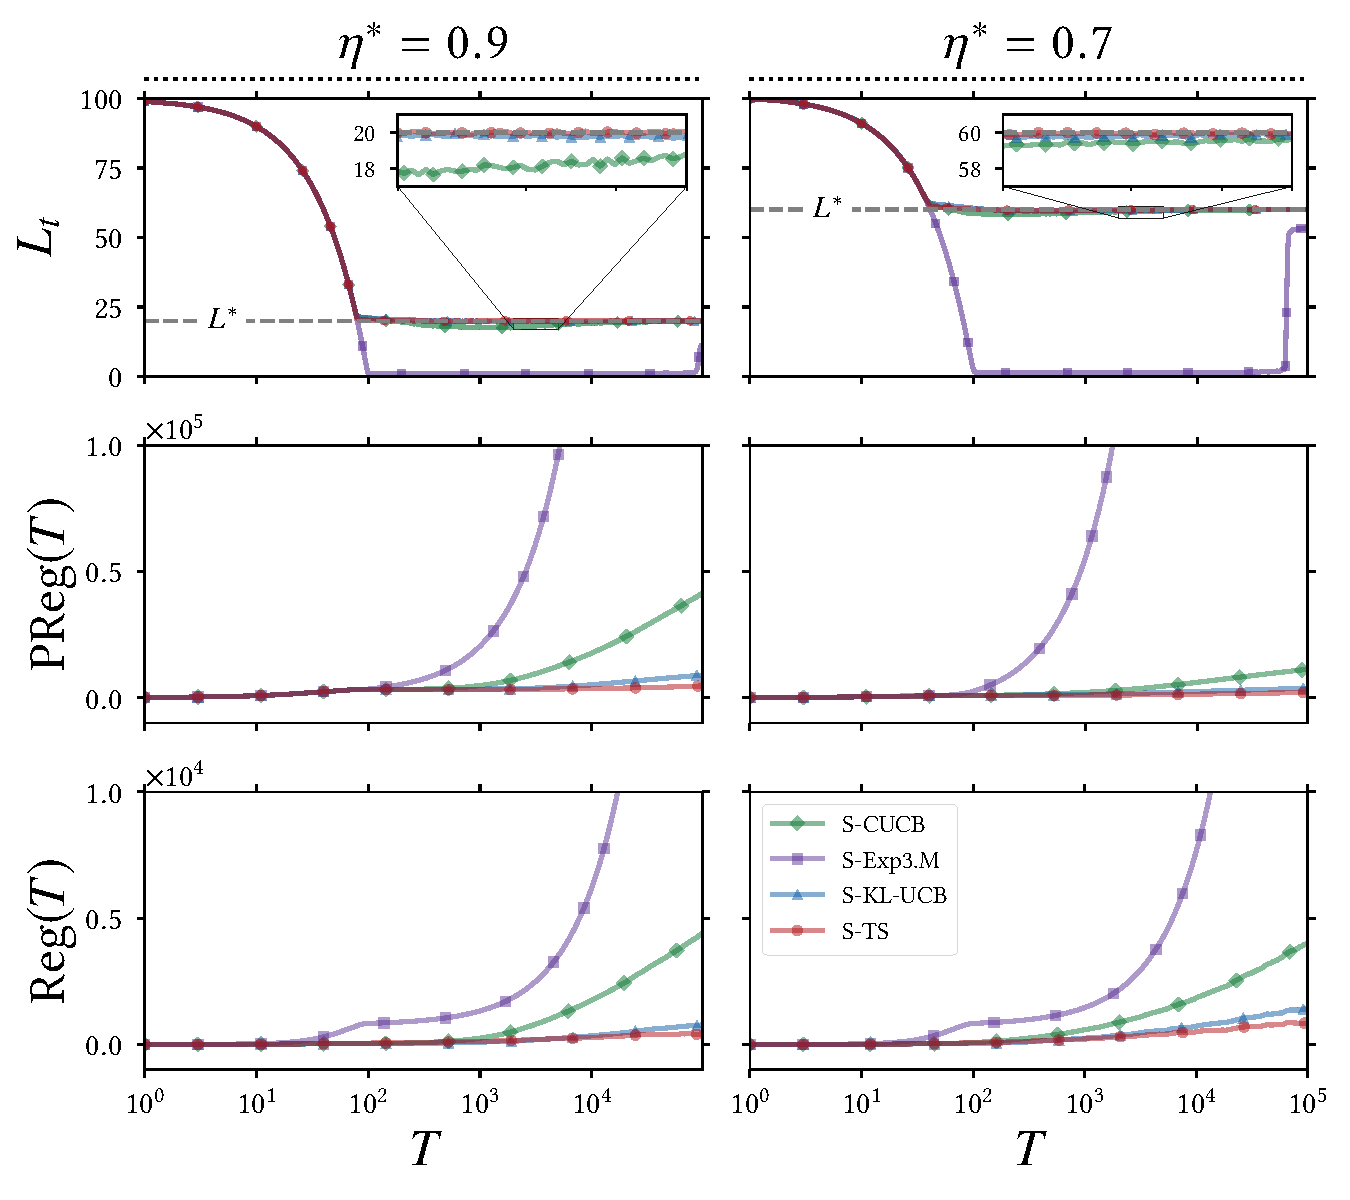
\includegraphics[width=0.9\linewidth, trim=0cm 0cm 0cm 0.0cm]{part3-figures/static_experiment_s-2-compressed.pdf}
\caption{Static experiment: \gls{S-TS} minimises both regrets.}
\label{static_experiment}
\end{figure}

\subsection{Non-Static Environment}
\label{sec_nonstatenv}

In this section, we want to verify whether \gls{S-TS-ADWIN} adapts to changes in the reward distribution. We compare our results against the following state-of-the-art non-static bandit algorithms: 
\begin{itemize}[noitemsep]
	\item \gls{dTS}  applies a discounting factor $\gamma$ to the parameter $\alpha_i$, $\beta_i$ of the Beta posterior for each arm $i \in \gls{K}$ at each time step $\gls{t}$. 
	\item \gls{EG} successively selects with probability $\epsilon$ the arm with the highest reward seen so far. Otherwise, it selects an arm randomly. \item \gls{SW-UCB} discards any information older than a sliding window of fixed size $\gls{w}$. 
\end{itemize}

We set $\gls{eta^*} = 0.6$ and use the previous static setup to generate our non-static scenarios. In line with the literature \cite{DBLP:journals/csur/GamaZBPB14}, we simulate `gradual' and `abrupt' changes: 
\begin{itemize}[noitemsep]
\item \textbf{Gradual}: We place 60 equidistant change points over the time axis. For the first 30 change points, we set $\mu_h = 0$ for the arm $h \in \gls{K}$ with the current highest expected reward. Then, we revert those changes in a `last in -- first out' way. 
Thus, $\gls{L^*}$ evolves gradually from $80$ to $20$, and back. 
\item \textbf{Abrupt}: We place two change points, equidistant from the start and end. 
At the first one, we set $\mu_h = 0$ for the top-$30$ arms. We revert this change at the second change point. 
Thus, $\gls{L^*}$ abruptly changes from $80$ to $20$ and back.
\end{itemize}

Since the environment is non-static, $\gls{mu_i}$ and $\gls{L^*}$ now vary as a function of $\gls{t}$. Thus, we measure regret against a piecewise static oracle, which `knows' $\gls{mu_i}(\gls{t})$ and $\gls{L^*}(\gls{t})$.

A key result from this experiment is that \gls{S-TS}, which assumes that arms do not change over time, fails to adapt to a changing environment. In contrast, our improvement, \gls{S-TS-ADWIN}, does (Fig\-ure~\ref{non-static-experiment-1}) and even outperforms all alternatives (Figure \ref{non-static-experiment-2}).

Figure \ref{non-static-experiment-1} shows that S-\gls{CUCB}(-\gls{ADWIN}) and \gls{S-KL-UCB}(-\gls{ADWIN}) behave similarly to \gls{S-TS}(-\gls{ADWIN}), but have slightly higher regret and pull regret. S-\gls{Exp3.M} has very high pull regret. 
Overall, we see that our adaptation based on \gls{ADWIN} made it possible to handle both gradual and abrupt changes.

\begin{figure}[ht]
	\centering
		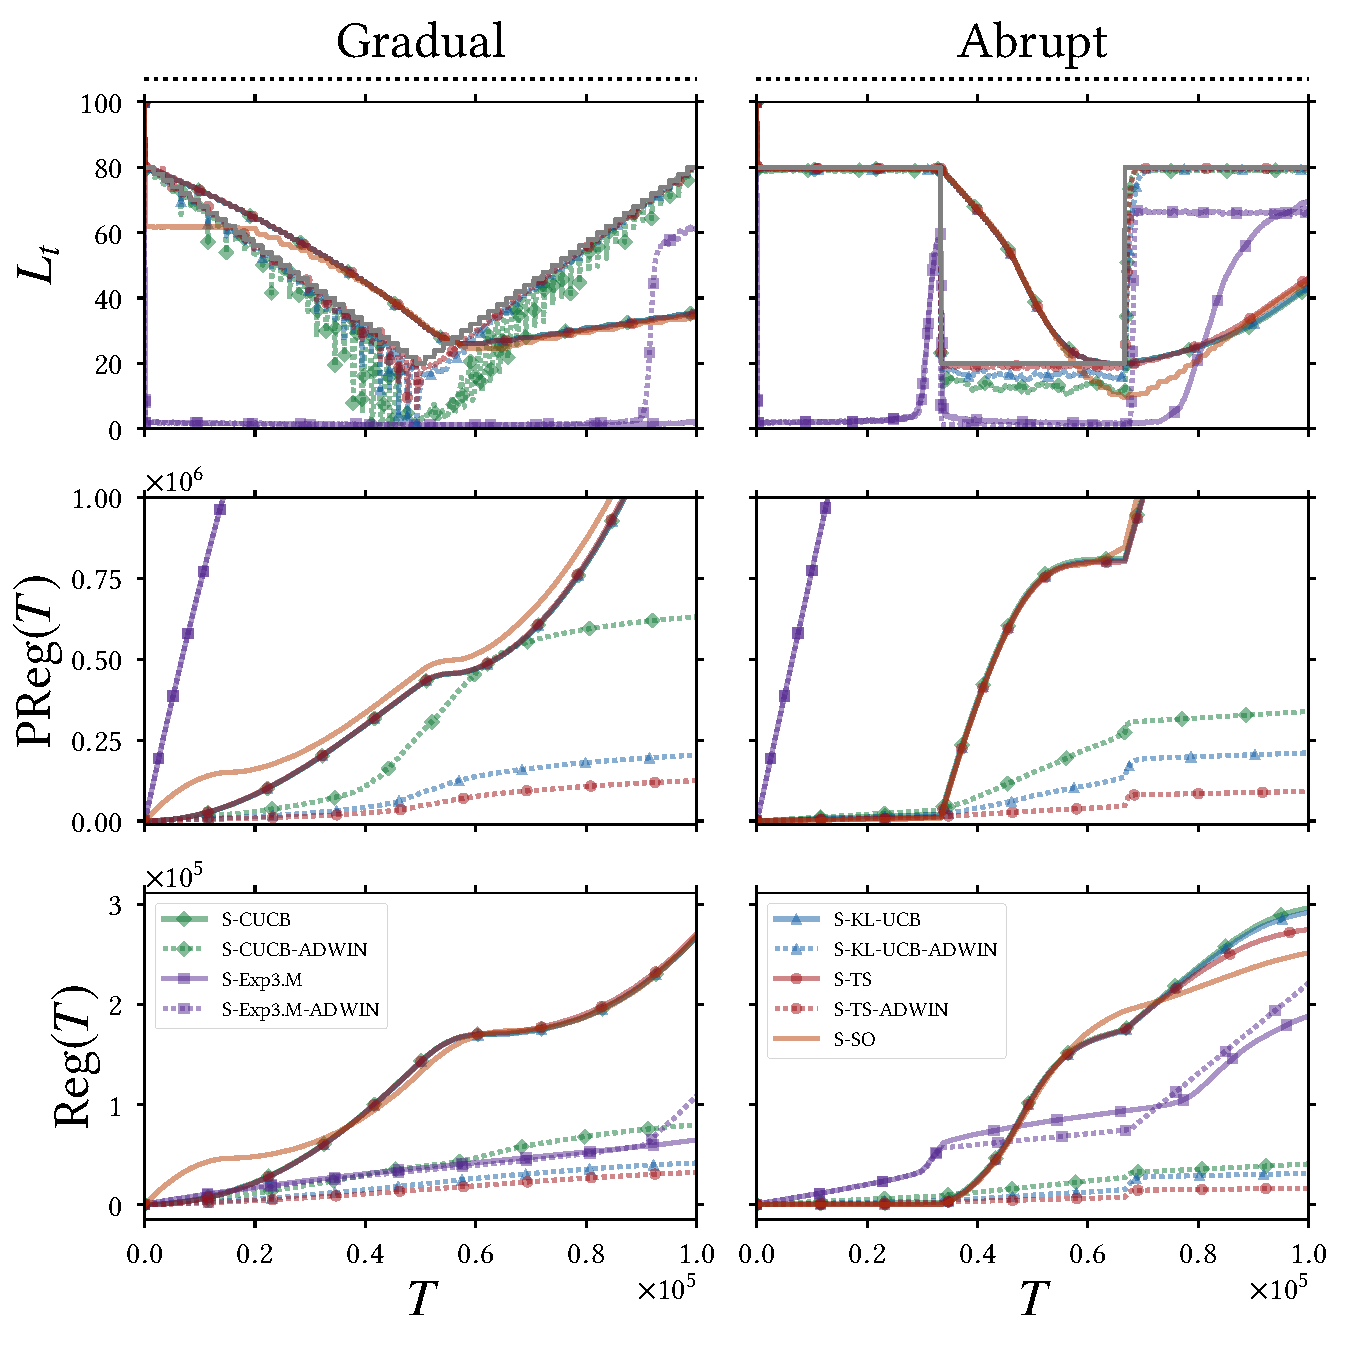
\includegraphics[width=0.9\linewidth, trim=0cm 0cm 0cm 0.5cm]{part3-figures/gradual_abrupt_regret_small-2-compressed.pdf}
	\caption{Non-static experiment: \acrshort{S-TS} vs. \acrshort{S-TS-ADWIN}.} 
	\label{non-static-experiment-1}
\end{figure}

Figure \ref{non-static-experiment-2} compares our approach to the existing non-static bandit alternatives. S-\gls{dTS} tends to underestimate $\gls{L^*}$ in the case of a strong discounting factor, e.g., for $\gamma = 0.7$. 
On the contrary, S-\gls{SW-UCB} overestimates $\gls{L^*}$, in particular when the window size $\gls{w}$ is small. \textsc{S-\gls{EG}} behaves similarly as the static approaches: it does not adapt to change quickly. 

We also see that \gls{S-TS-ADWIN} is robust for a large range of $\delta$, except for very small values, e.g., $0.01$ and $0.001$. The best results are obtained with $\delta = 0.1$, which is consistent with the results in \cite{DBLP:conf/sdm/BifetG07}. 
Other approaches, in turn, are quite sensitive to their parameters. 
For example, we can see that a weak discounting factor of $\gamma = 0.99$ is beneficial for \gls{dTS} in the case of a gradual change, but that more aggressive discounting is better with abrupt changes. 
The figure shows that our approach adapts to different kinds of change, as opposed to the other approaches, without tuning its parameter. 
\begin{figure}[ht]
	\centering
		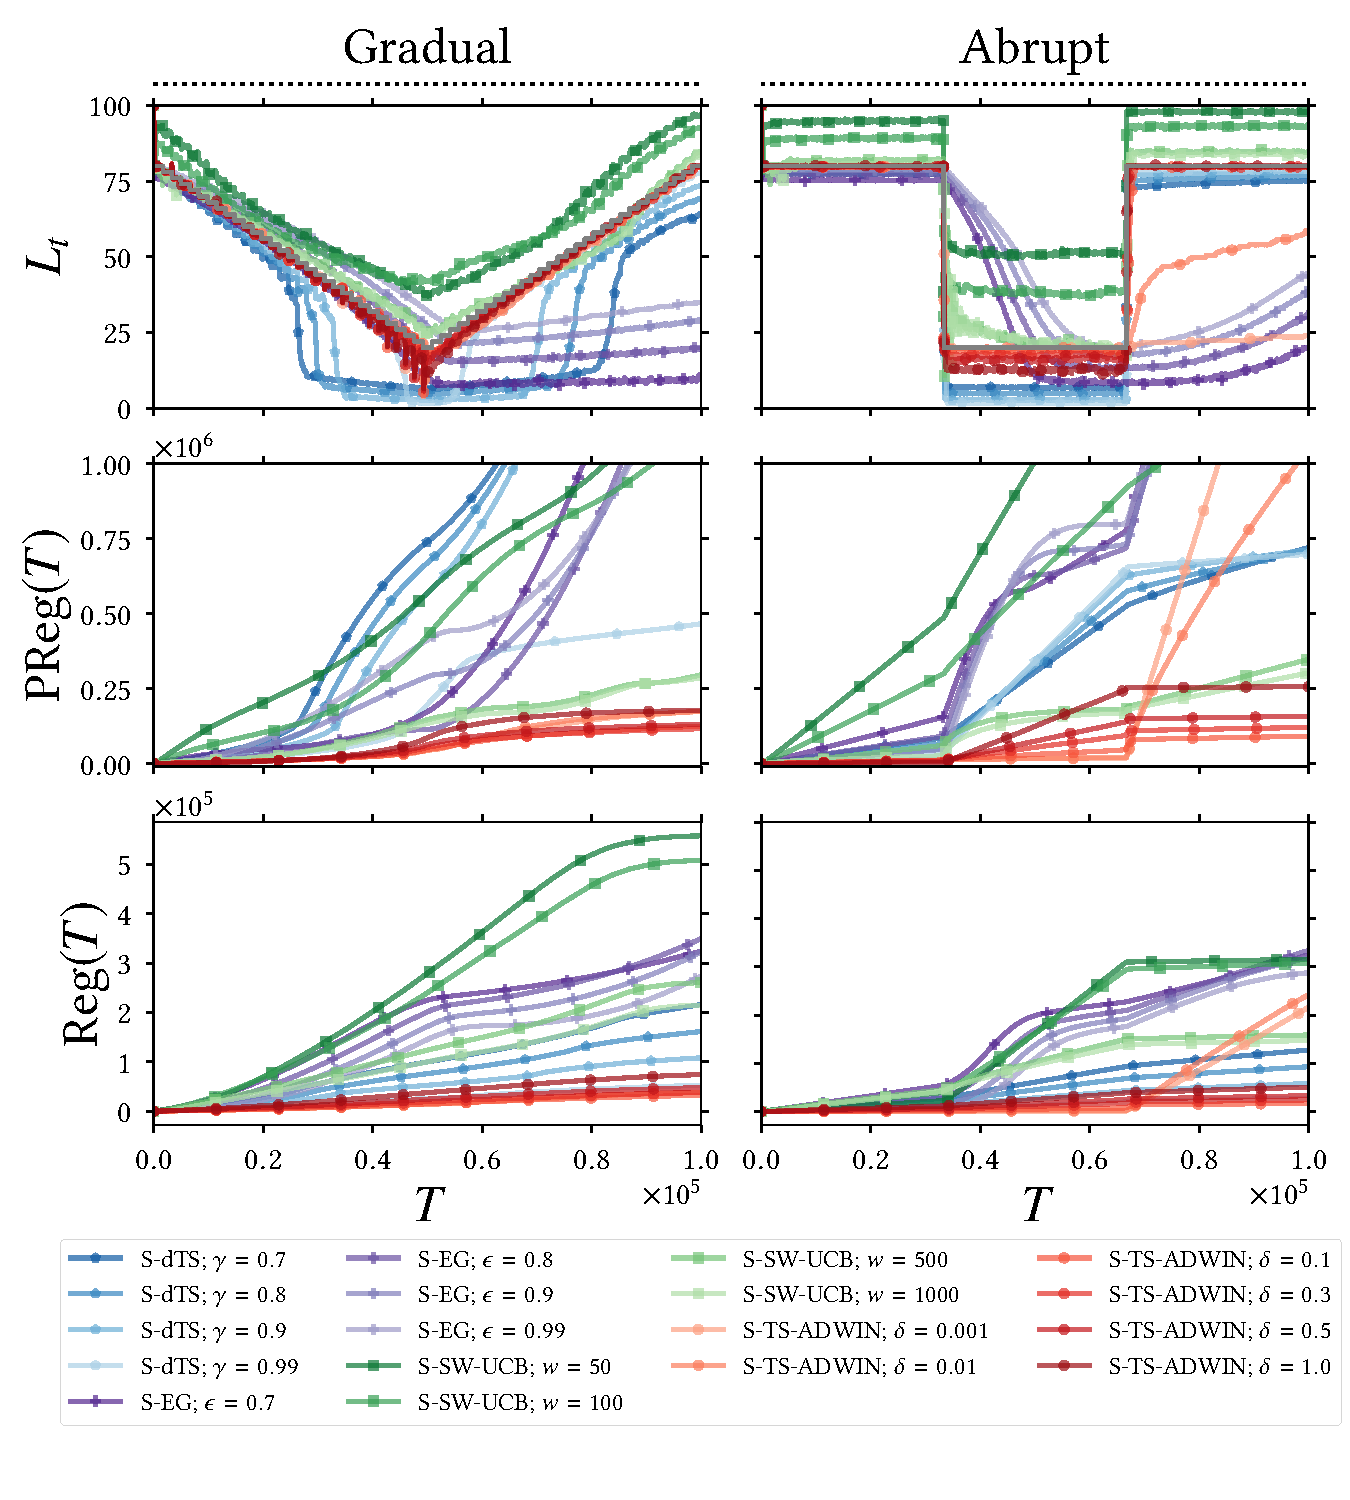
\includegraphics[width=0.85\linewidth, trim=0cm 0cm 0cm 0.5cm]{part3-figures/gradual_abrupt_regret_long-2-compressed.pdf}
	\vspace{-0.8cm}
	\caption{Non-static experiment: Non-static bandits.} 
	\label{non-static-experiment-2}
\end{figure}

\subsection{Case Study: Monitoring Dependency}
\label{sec_streammonitoring}

\glsunset{Bioliq}
In this section, we look at our real-world example: the \gls{Bioliq} power plant. We create a data set corresponding to a week of measurements.
It contains one measurement per second from a selection of 20 sensors, such as temperature, pressure, in various components. 

We consider \gls{MI} \cite{kraskov2004estimating} as a measure of correlation, which we have computed pair-wise between all attributes over a sliding window of size $1000$ ($\sim$ 15 minutes) with step size $100$ ($\sim$ 1.5 minute).
Our goal in this use case is to employ bandit algorithms as a `monitoring system' to keep an overview of large correlation values in the stream. Whenever the monitoring system detects a \gls{MI} value higher than a threshold $\Gamma$, it obtains a reward of $1$, otherwise $0$. 
The challenge is to decide which coefficients to re-compute and how many of them at each step. 
This results in a \gls{S-MAB} problem with 6048 steps and $(20*19)/2 = 190$ arms. 

Figure \ref{rewardmatrix} is the reward matrix for $\Gamma = 2$. 
We see that there are fewer rewards at the beginning and end of time.
This is because the week is bordered by periods of lower activity in the plant. In the weekends, we observe fewer correlations than during weekdays. 

\begin{figure}
	\begin{center}
		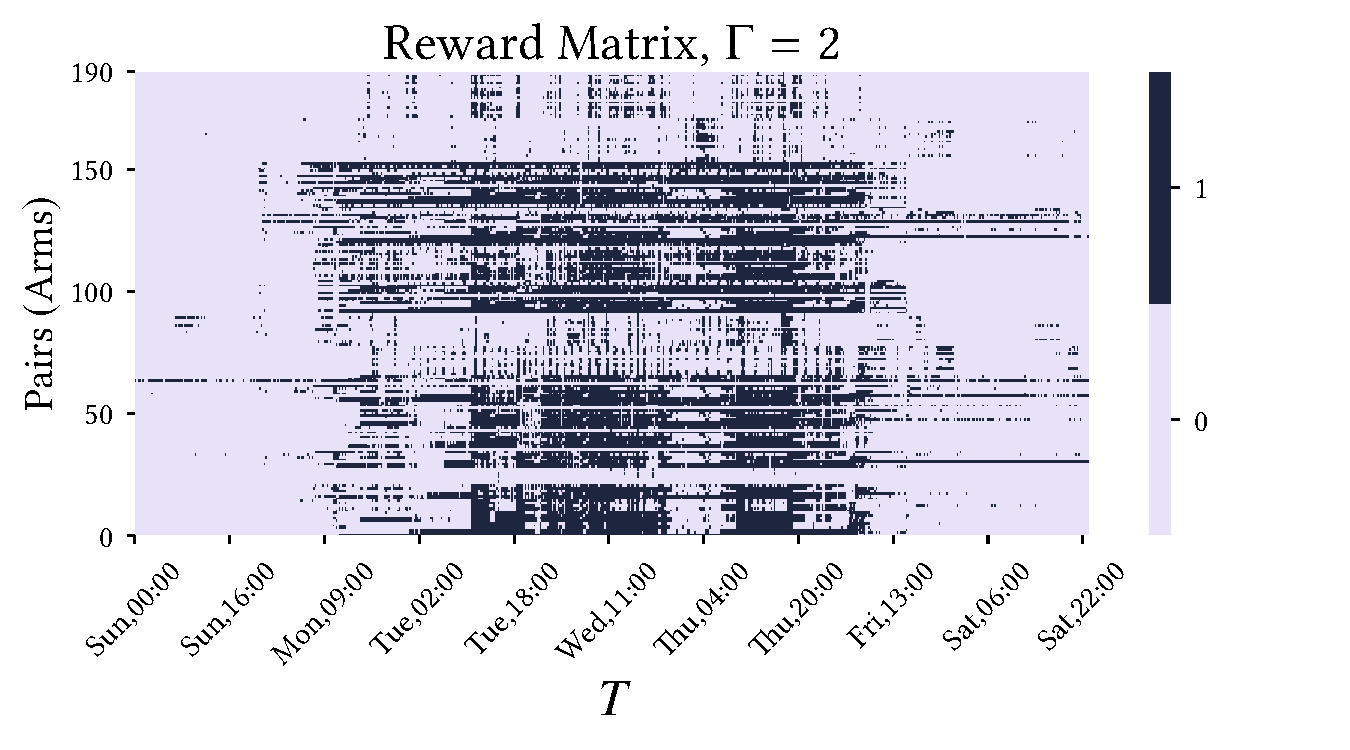
\includegraphics[width=1.0\linewidth, trim=0cm 0cm 2cm 0cm]{part3-figures/reward_heatmap_bioliq_1wx20_100-2-compressed.pdf}
	\end{center}
	\vspace{-1cm}
	\caption{Real-world experiment: Distribution of rewards.} 
	\label{rewardmatrix}
\end{figure} 

Since there is no ground truth $\{\gls{mu_i}(\gls{t})\}$, it is not possible to assess the pull regret nor the standard regret. 
Instead, we compare the rewards and costs across algorithms: 
whenever an Algorithm A obtains more rewards than an Algorithm B for the same cost (i.e., number of plays), we conclude that A is superior to B.  
We compare against oracles with different levels of knowledge: \gls{RO},  \acrfull{SO} and \gls{DO} are shown as a black, green and gold dotted lines respectively. 

In Figure \ref{real_world_experiment_Lt}, we set $\gls{eta^*} = 0.8$ and visualise the evolution of the number of plays over time for various approaches. 
\gls{S-TS-ADWIN} is the closest match to S-\gls{DO}-\gls{ADWIN}, our strongest baseline. This indicates that \gls{S-TS-ADWIN} adapts to changes of rewards to find a proper value for ${\gls{T}}$, unlike static algorithms such as \gls{S-TS}.

\begin{figure}
	\begin{center}
		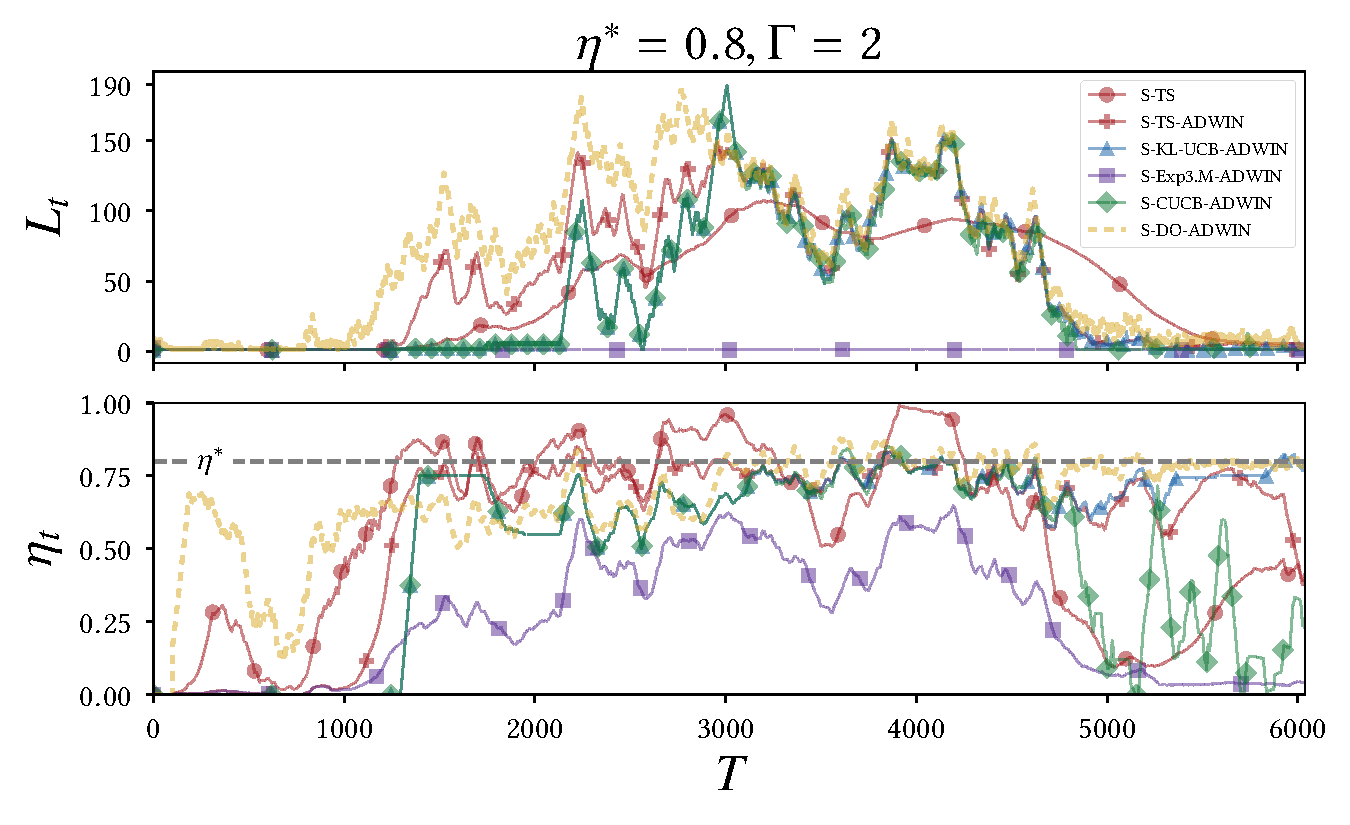
\includegraphics[width=1.0\linewidth]{part3-figures/Lt_etat-2-compressed.pdf}
	\end{center}
	\caption{Real-world experiment: Variation of ${\gls{T}}$ and $\eta_t$.} 
	\label{real_world_experiment_Lt}
\end{figure} 

\begin{figure}
	\centering
	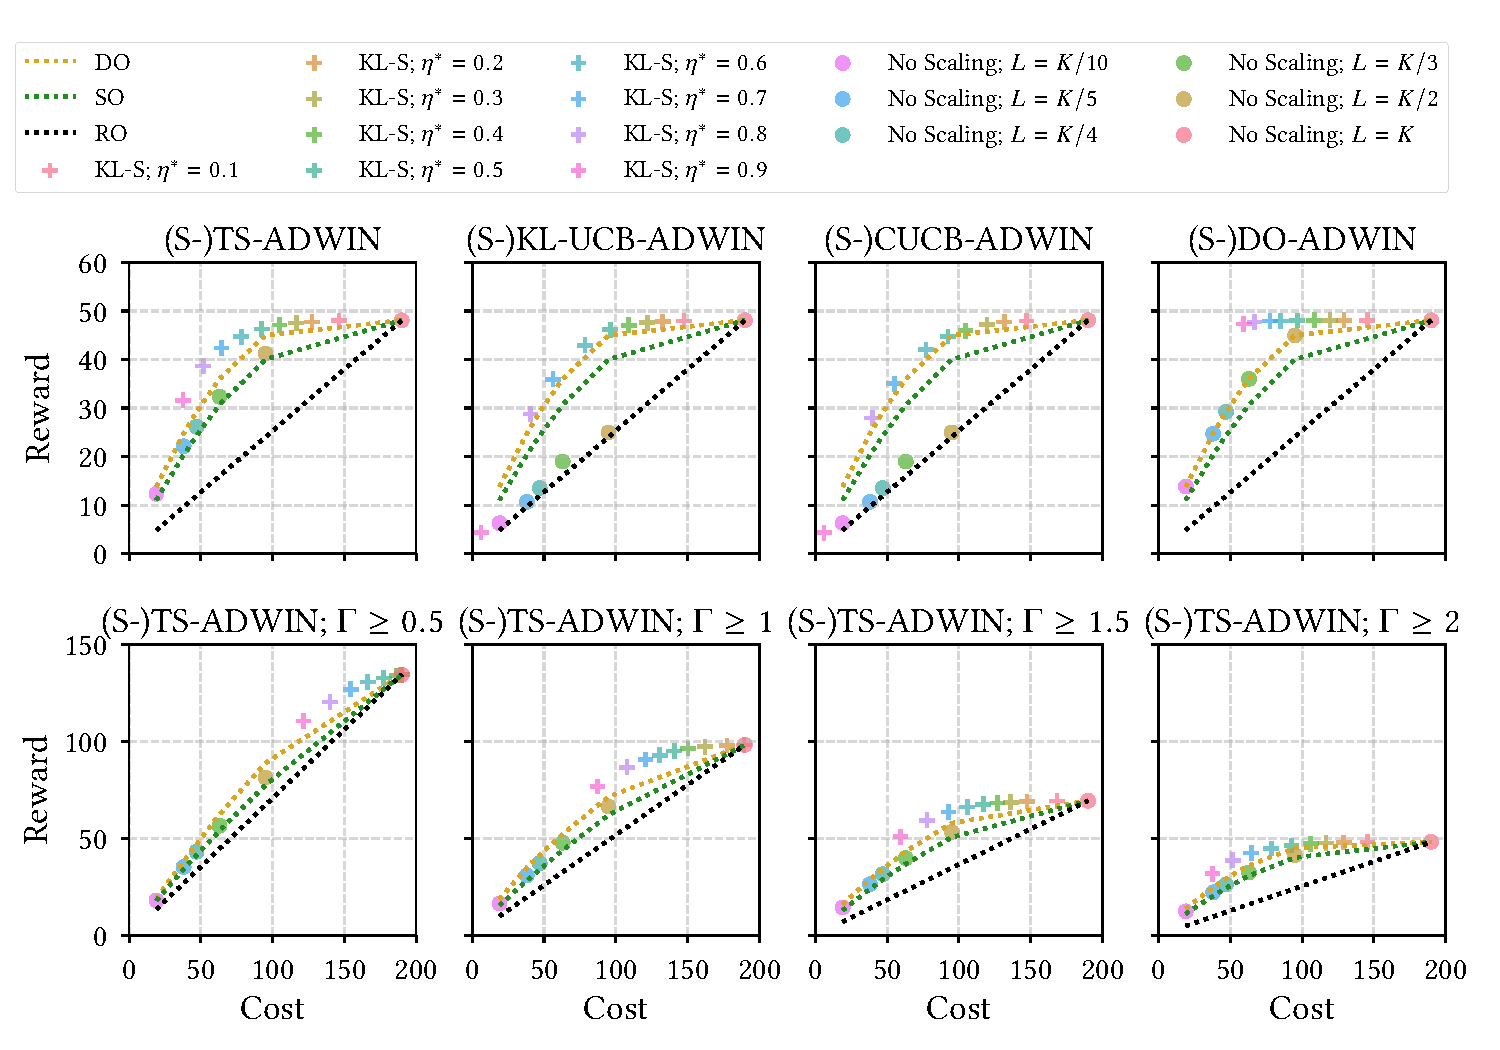
\includegraphics[width=1.0\linewidth]{part3-figures/RealWorld_2_legend-2-compressed.pdf}
	\caption{Real-world experiment: Scaling versus No Scaling.}
	\label{real_world_utility}
\end{figure} 

Figure \ref{real_world_utility} shows the relationship between the average reward and the average cost (in terms of number of plays) of each algorithm. 
\gls{S-TS-ADWIN} consistently yields higher rewards than \gls{DO} for the same costs. 
\gls{TS}-\gls{ADWIN} (without scaling) also is superior to \gls{SO}. Here we see the full benefit of our scaling policy with S-\gls{DO}-\gls{ADWIN}: 
the scaling dynamic oracle consistently achieves nearly maximal reward, while pulling fewer arms than a non-scaling algorithm. In other words, it outperforms its non-scaling counterpart. 

Surprisingly, the \gls{UCB}-based approaches do not perform well without scaling; they are close to the \acrfull{RO}. We hypothesise that \gls{ADWIN} keeps the size of the dynamic window small in the real-world setting; $\gls{w}_{\gls{t}}$ remains small, affecting the sharpness of the confidence bound. However, when our scaling policy is used, both approaches perform slightly better than \gls{DO}. 

We also verify that \gls{S-TS-ADWIN} can adapt to different environments by changing $\Gamma$, which influences the availability of rewards. 
We see here that the improvement against our baselines is consistent, i.e., our algorithm also adapts the number of plays per round. 

Finally, we evaluate the scalability of our approach w.r.t. $\gls{K}$ and $\gls{T}$. 
To do so, we stick to our real-world example and create versions of the problem of different size with $10$ to $2000$ arms and up to $10^5$ steps, by resampling the arms and observations. Then, we run our real-world experiment with $\Gamma = 2$ and average the runtime with scaling parameter $\gls{eta^*}$ from $0.1$ to $0.9$. Figure~\ref{real_world_scalability} shows the result. 

We see that each bandit approach scales linearly with the number of arms and the number of steps. S-\gls{CUCB} is the fastest one, closely followed by \gls{S-TS} and \gls{S-KL-UCB}. 
S-\gls{Exp3.M} is two orders of magnitude slower w.r.t. $\gls{K}$. 
By comparing \gls{S-TS} and \gls{S-TS-ADWIN}, we see that the added computational burden from \gls{ADWIN} is small and scales alike with an increasing number of arms and time steps.
Each bandit approach, except \gls{Exp3.M}, is at most one order of magnitude slower than choosing arms at random (\gls{RO}). We see that our approach requires on average one millisecond to decide which arms to play when $\gls{K}=100$.
This is typically less than the time required at each step to estimate \gls{MI} on a single pair, using state-of-the-art estimators \cite{kraskov2004estimating}.

Altogether, our experiments verified that our algorithms, \gls{S-TS} and \gls{S-TS-ADWIN}, are both effective and efficient. \gls{S-TS} outperforms state-of-the-art bandits in the static setting, while \gls{S-TS-ADWIN} adapts better to different kinds of change than its competitors. In our real-world example, \gls{S-TS-ADWIN} obtains almost all the rewards in the environment for a cost reduced by up to 50\%, outperforming very competitive baselines, such as a non-scaling dynamic oracle. 

\begin{figure}
	\centering
	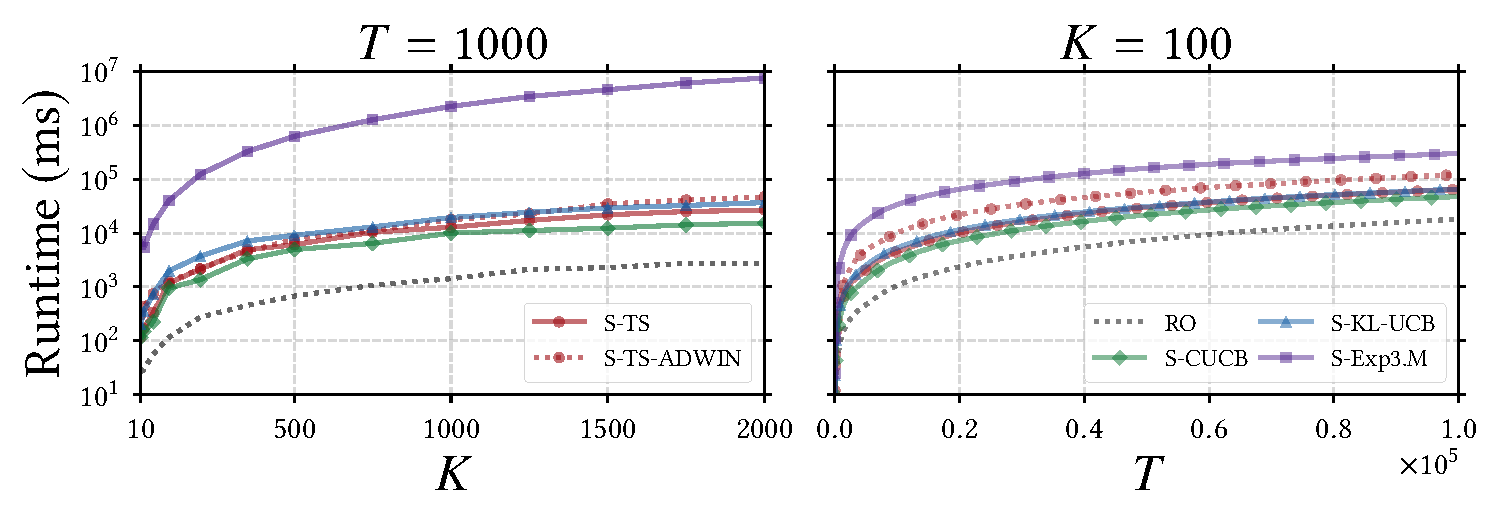
\includegraphics[width=0.9\linewidth]{part3-figures/scalability_decision_time-2-compressed.pdf}
	\caption{Scalability of bandit algorithms w.r.t. $\gls{K}$ and $\gls{T}$.} 
	\label{real_world_scalability}
\end{figure} 

\section{Discussion}
\label{conclusion}

We have proposed a new algorithm, \gls{S-TS}, which combines \acrfull{MP-TS} with a strategy to decide on the number of arms played per round, a so-called `scaling policy'.
Our analysis and experiments showed that it enjoys strong theoretical guarantees and very good empirical behaviour. 
We also proposed an extension of our algorithm for the non-static setting.
%, by combining it with \textsc{ADWIN}, a state-of-the-art change detector. 
We applied the proposed model to data stream monitoring and showed its utility. However, we expect the impact of our contribution to extend beyond this one application. In the next part, we discuss applications to Knowledge Discovery in high-dimensional data streams. 